% Figures
%\afterpage{
    \begin{figure}[t!]
        \centering
        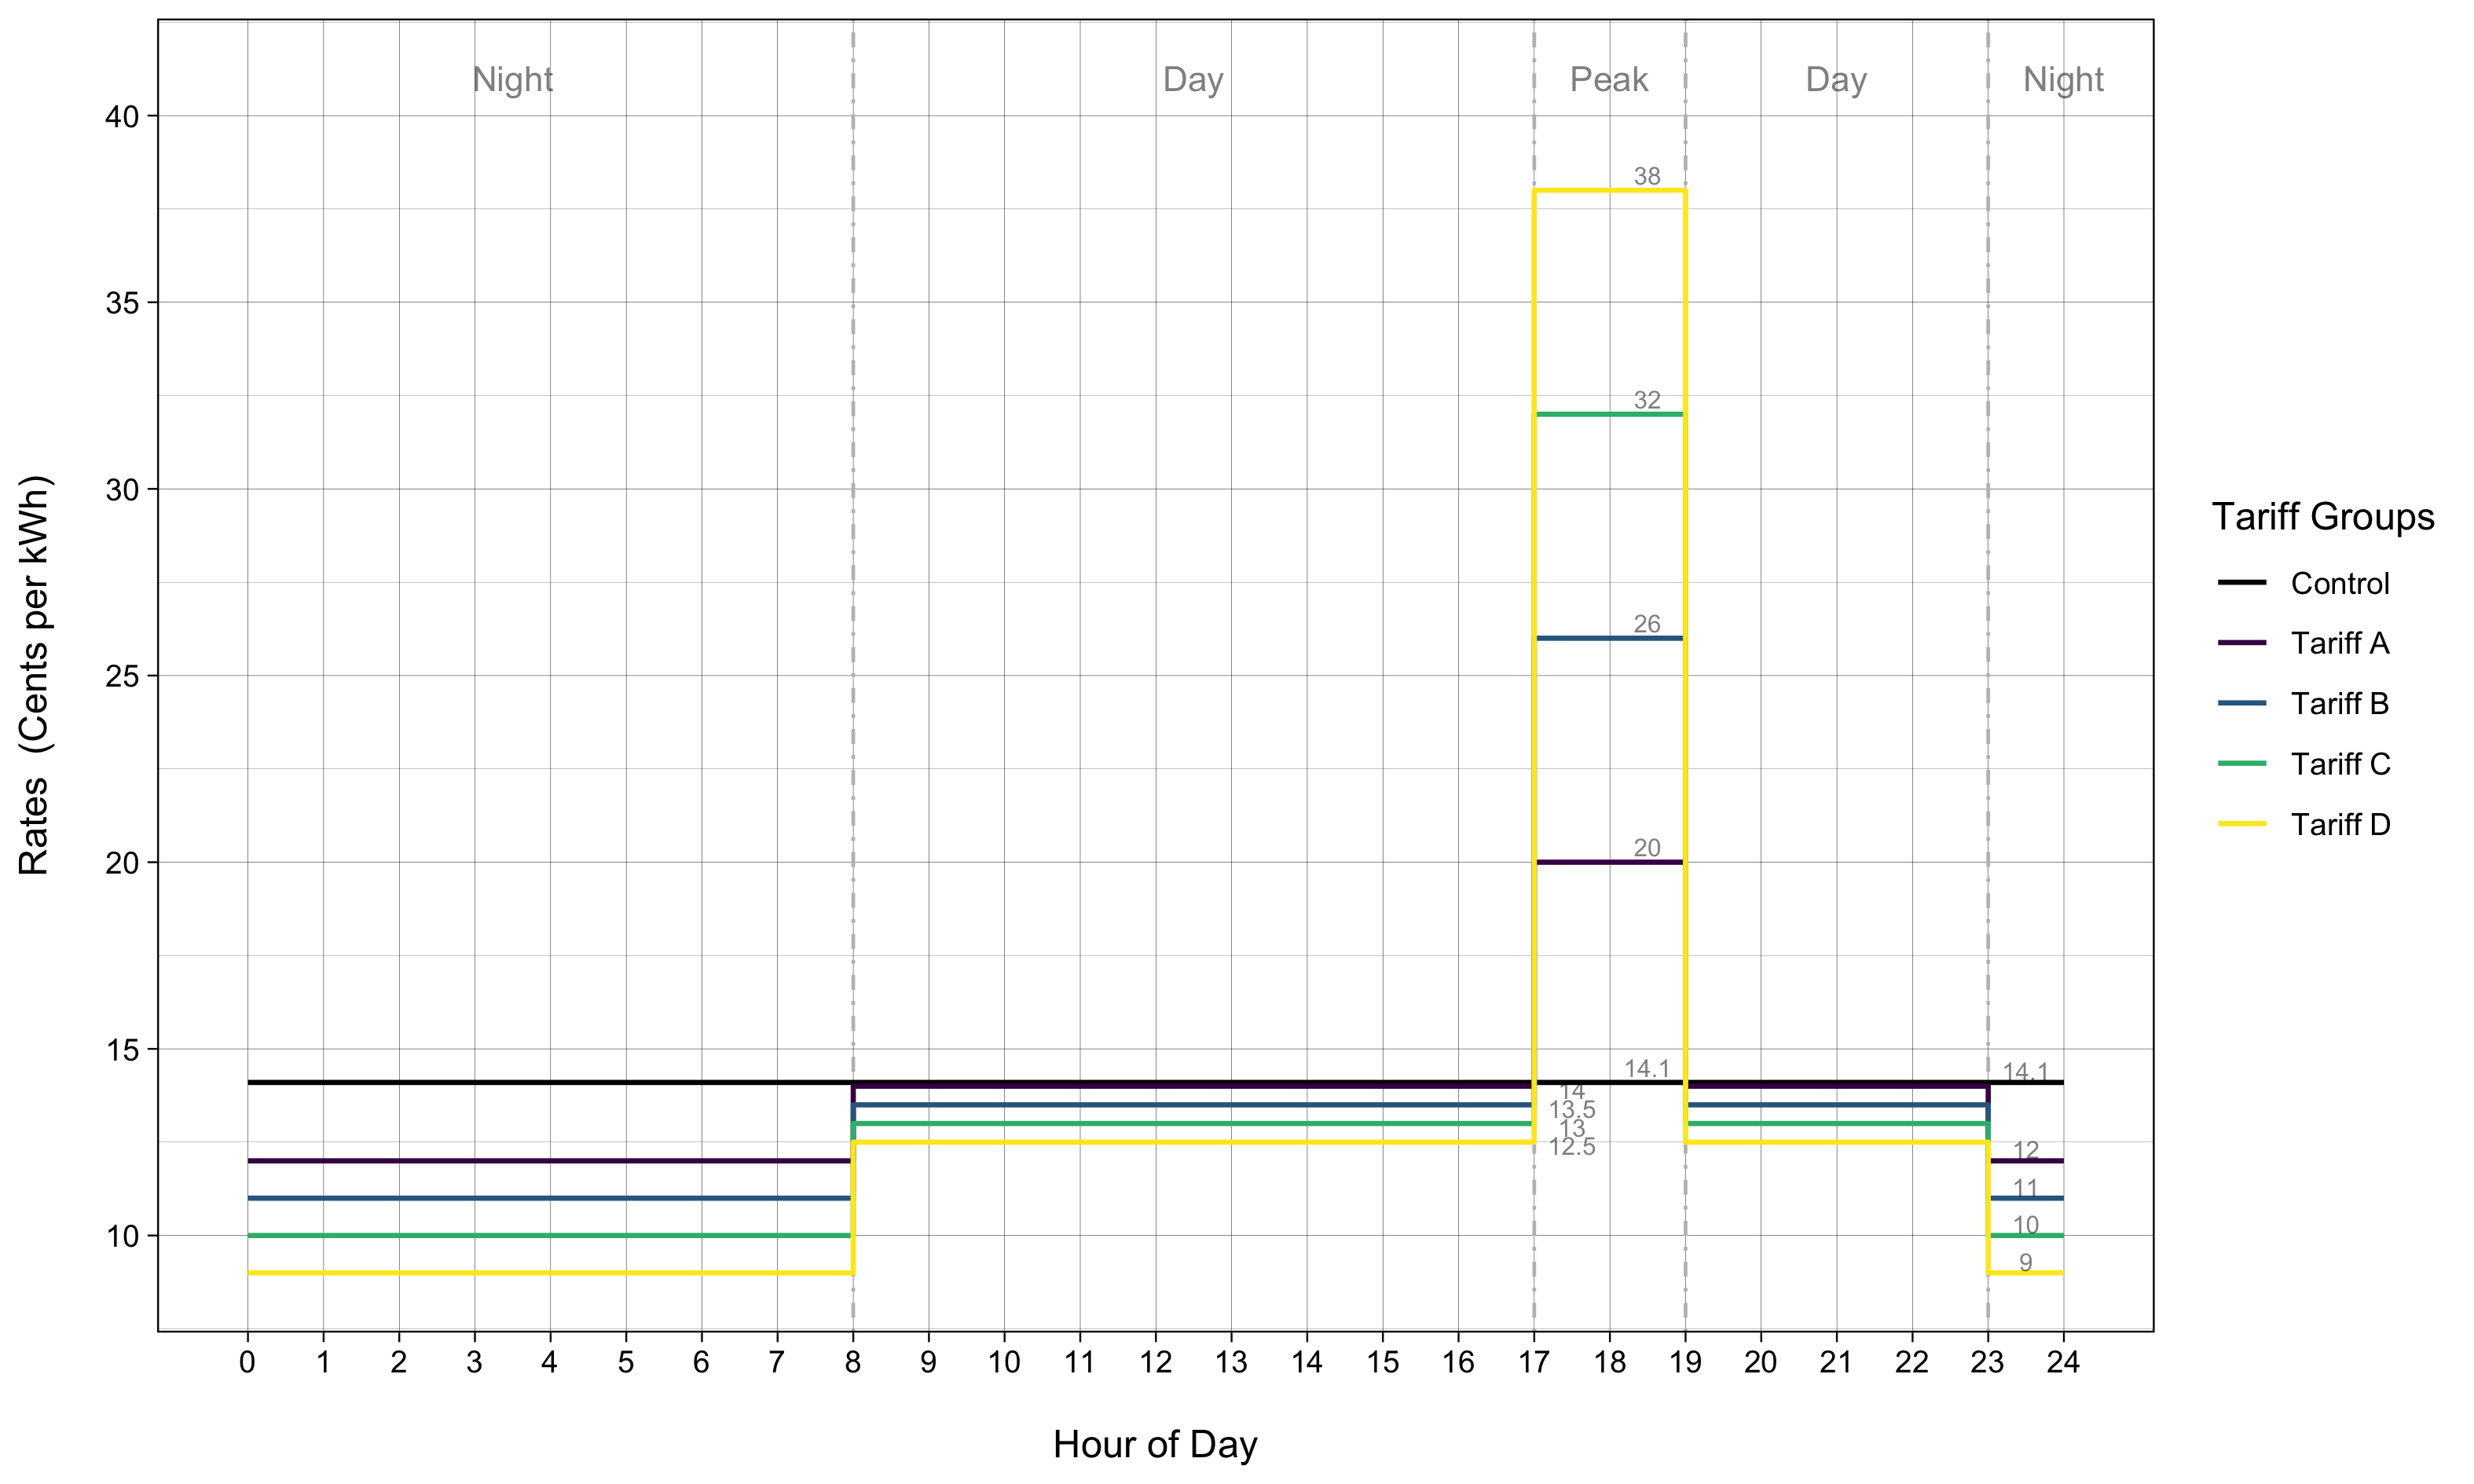
\includegraphics[scale = 0.13]{03_Chapter-2/00A_Figures/Figure_Time-of-Use-Tariff-Structures}
        \caption{Time-Of-Use Pricing Structures}
        \subcaption*{\textit{Note}: This figure illustrates the CER experiment in terms of TOU electricity pricing. The households in the control group were subject to a flat rate (i.e., 14.1 cents per kWh) during the entire experiment period. On the contrary, the treated households are assigned to one of four TOU tariff groups. And for each tariff group, there were three rate periods: night, day, and peak. Only the unit rate in the peak rate period was higher than the flat rate.}
        \label{Figure:Time-Of-Use-Pricing-Structures}
    \end{figure}
%}
%\clearpage
\hspace{0.3cm}

%\afterpage{
    \begin{figure}[ht!]
        \centering
        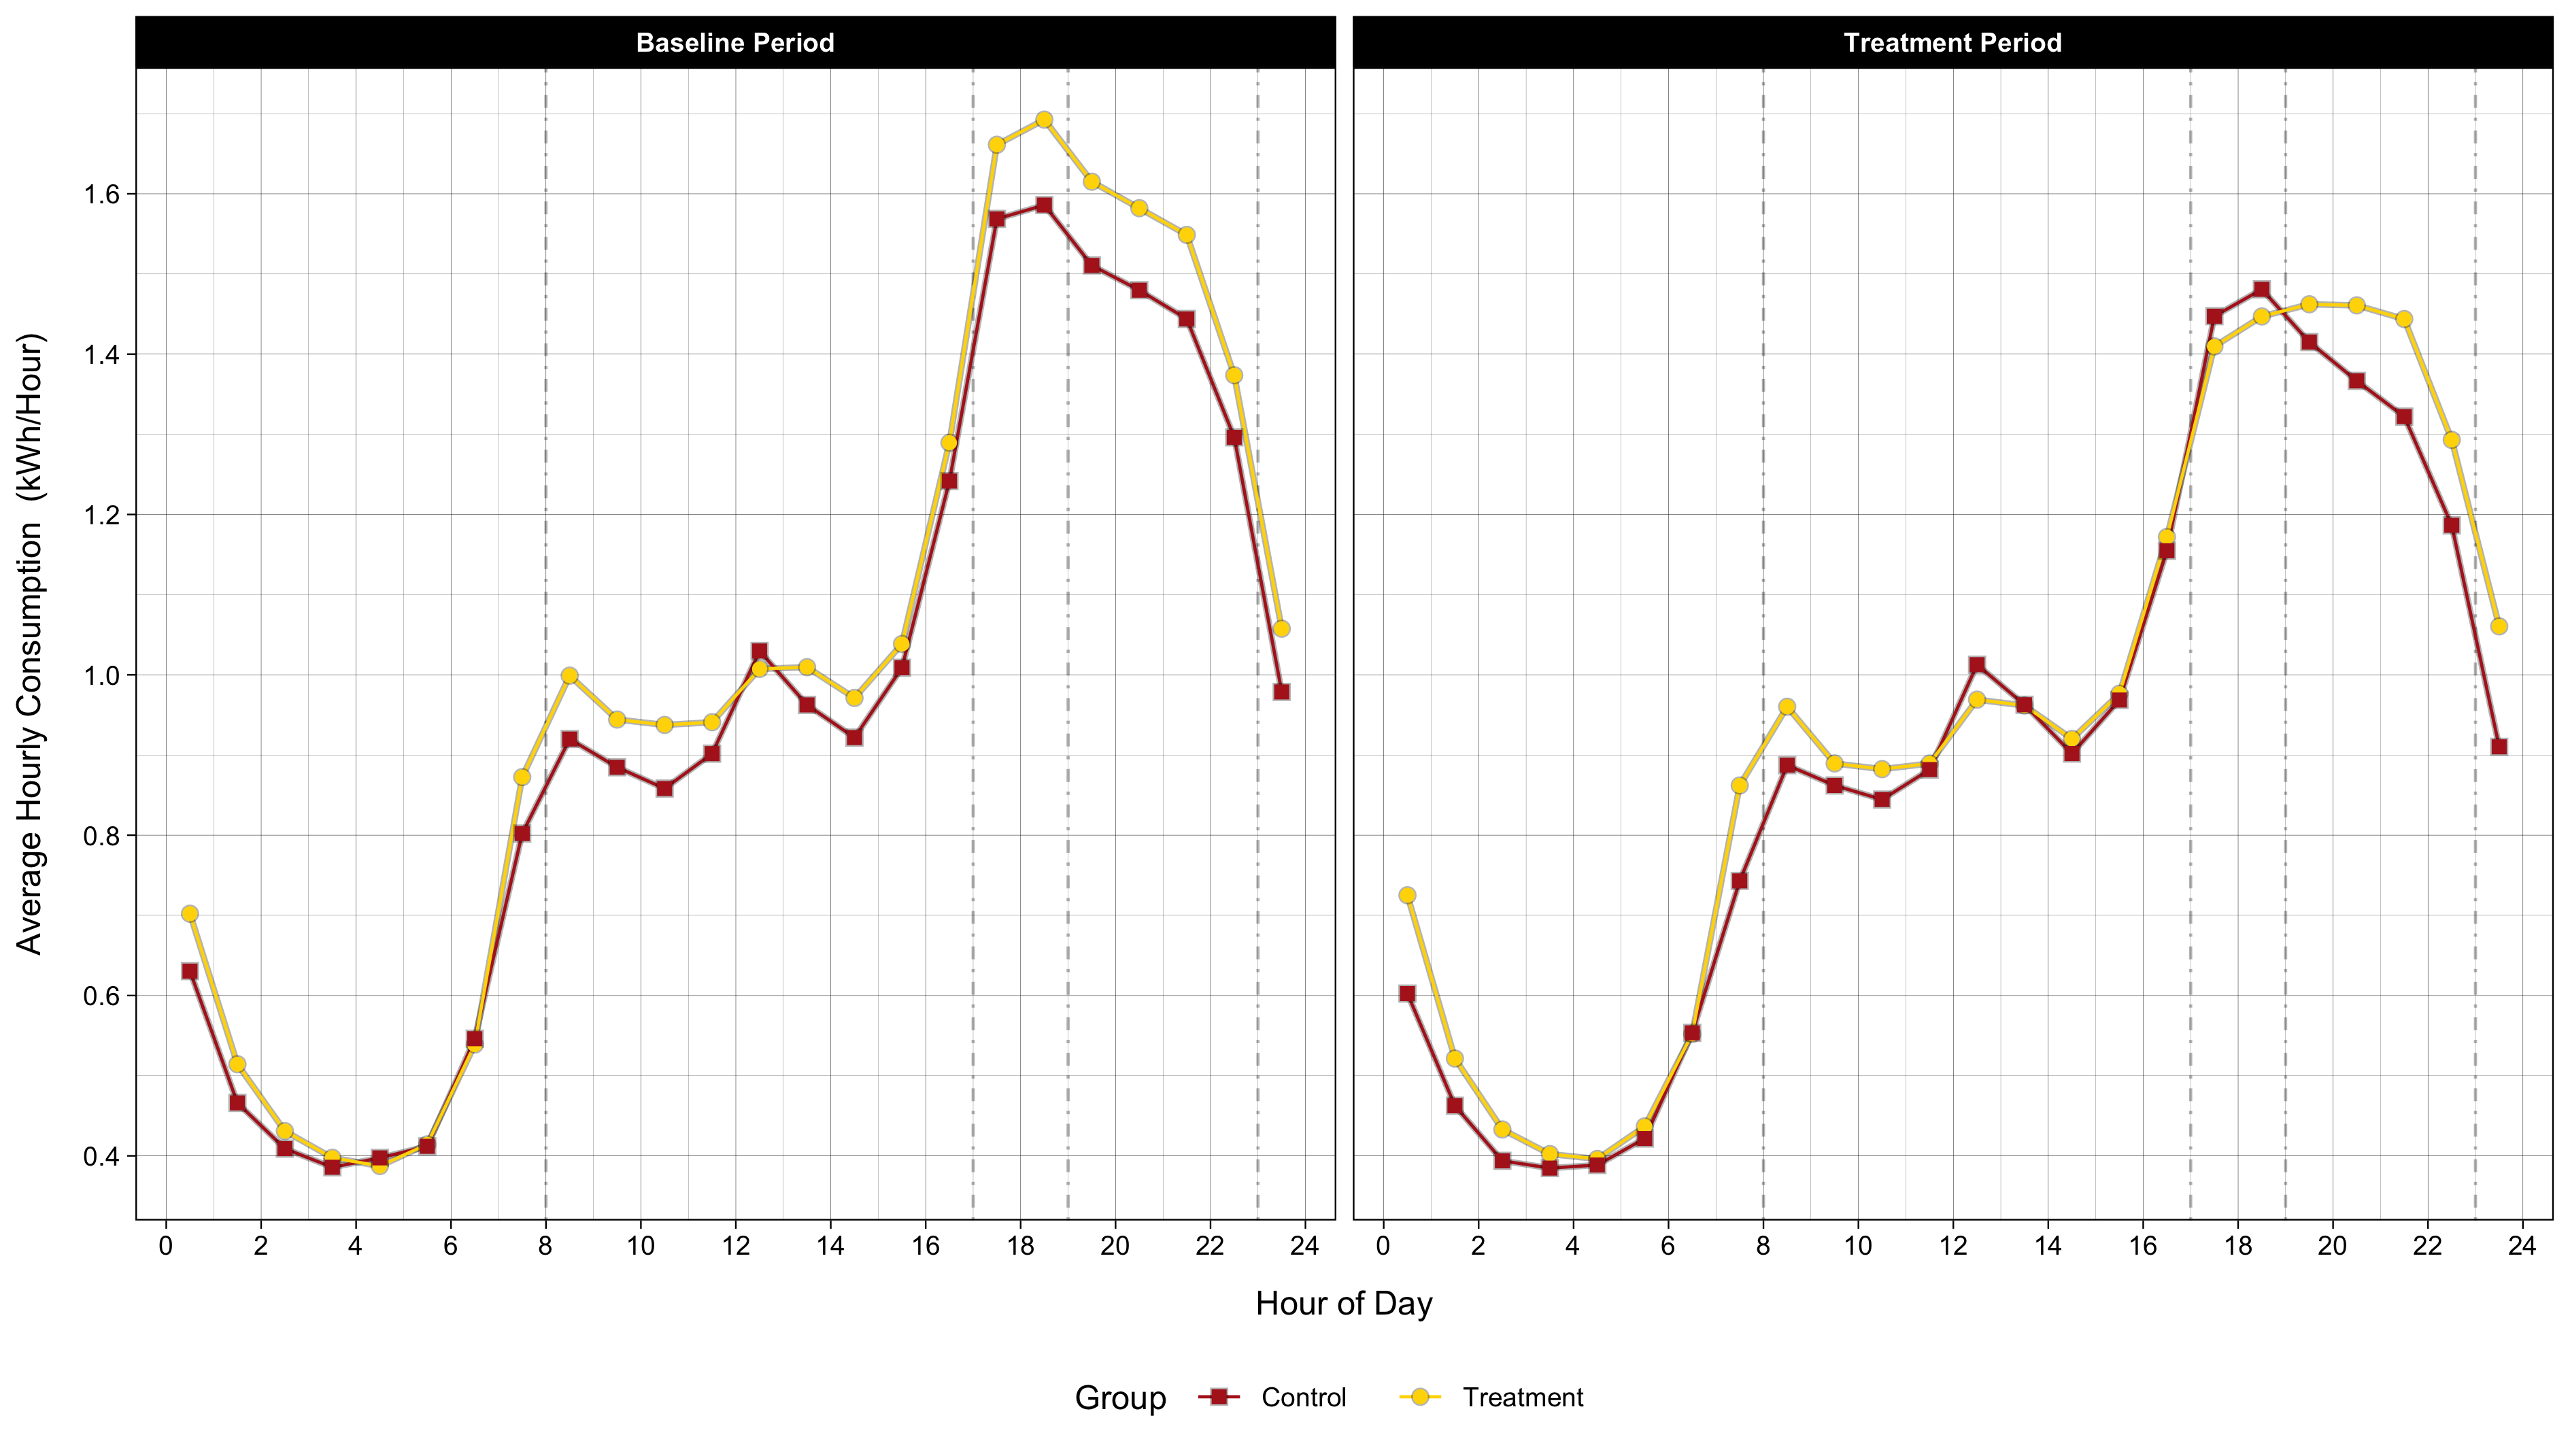
\includegraphics[scale = 0.1]{03_Chapter-2/00A_Figures/Figure_Average-Electricity-Consumption_Within-Day-Average-Hourly-Consumption.png}
        \caption{Average Hourly Electricity Consumption by Time of Day}
        \subcaption*{\textit{Note}: The figure shows household average hourly electricity consumption in the baseline and treatment periods. In general, during the baseline period, the treated households consumed more electricity at a given hour of the day. After introducing TOU tariff structures, they remarkably reduced their consumption in the peak rate period.}
        \label{Figure:Average-Hourly-Electricity-Consumption-by-Time-of-Day}
    \end{figure}
%}
\clearpage

%\afterpage{
    \begin{figure}[t!]
        \centering
        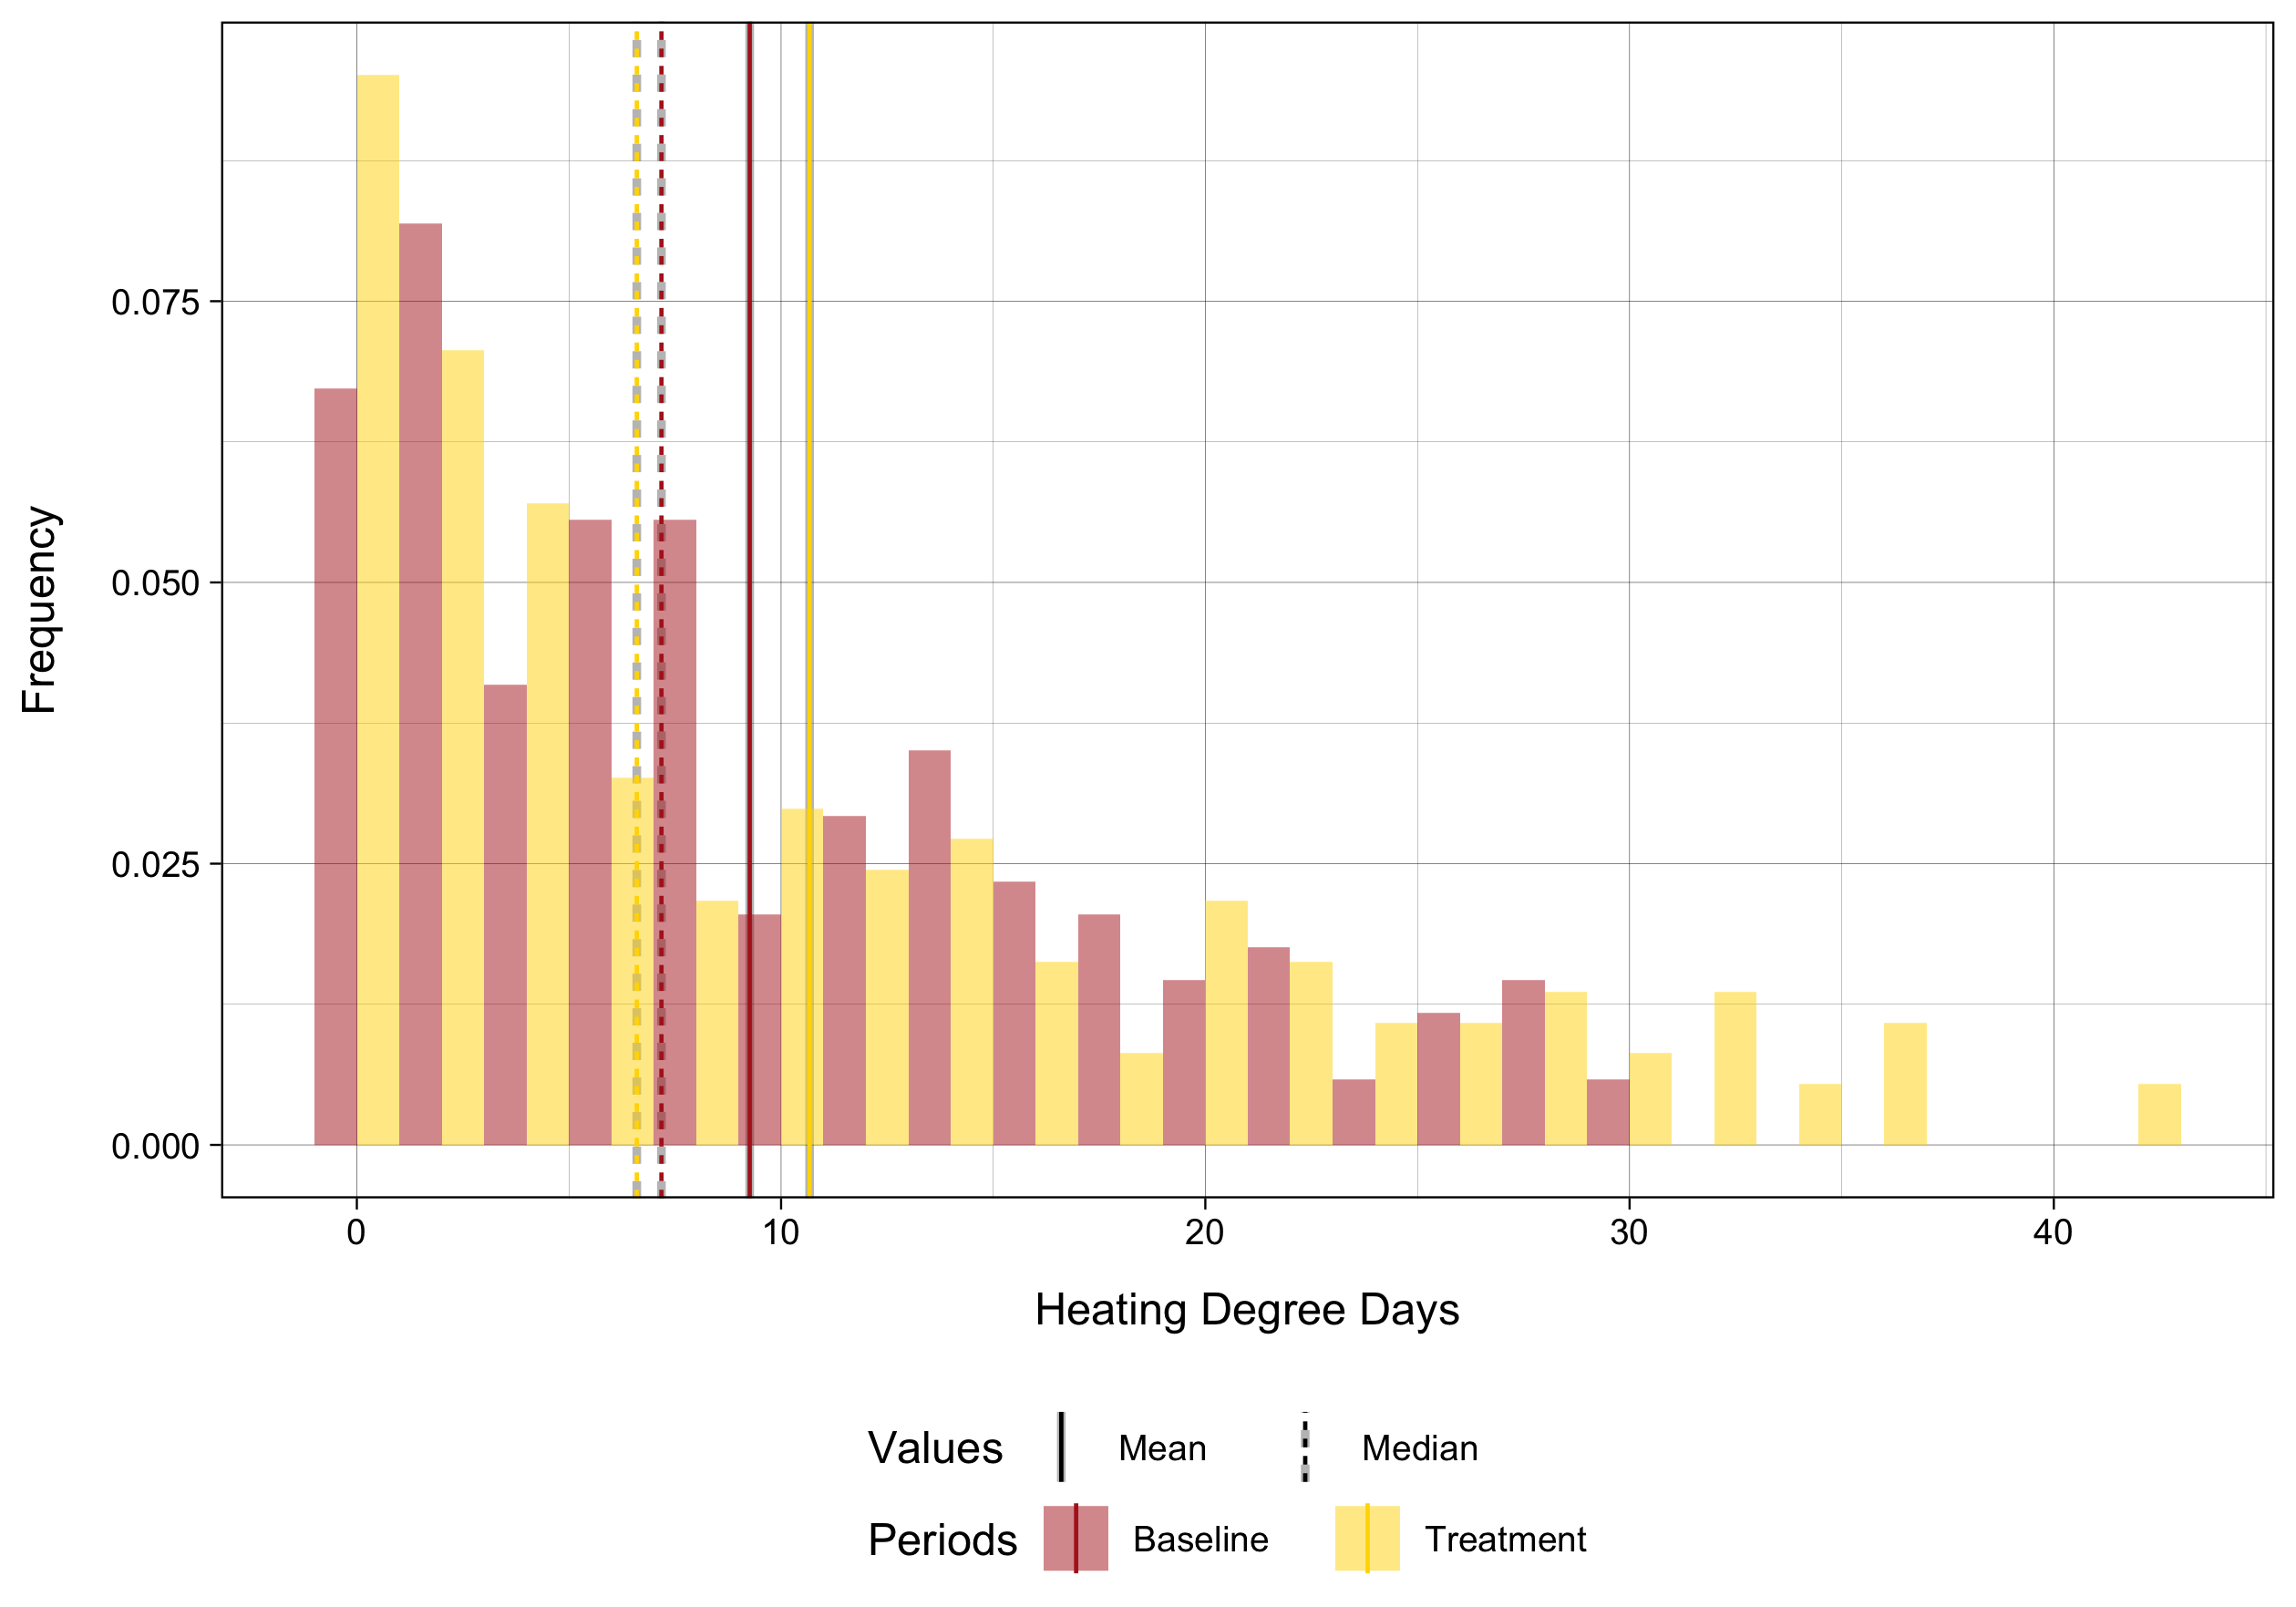
\includegraphics[scale = 0.155]{03_Chapter-2/00A_Figures/Figure_Distribution-of-HDDs.png}
        \caption{Distribution of Heating Degree Days during the Experiment Period}
        \subcaption*{\textit{Note}: This histogram shows the distribution of HDDs in each experiment period. Only the second halves are utilized to generate the histogram.}
        \label{Figure:Distribution-of-Heating-Degree-Days-during-the-Experiment-Period}
    \end{figure}
%}
%\clearpage
\hspace{0.3cm}

%%\afterpage{
%    \begin{figure}[ht!]
%        \centering
%        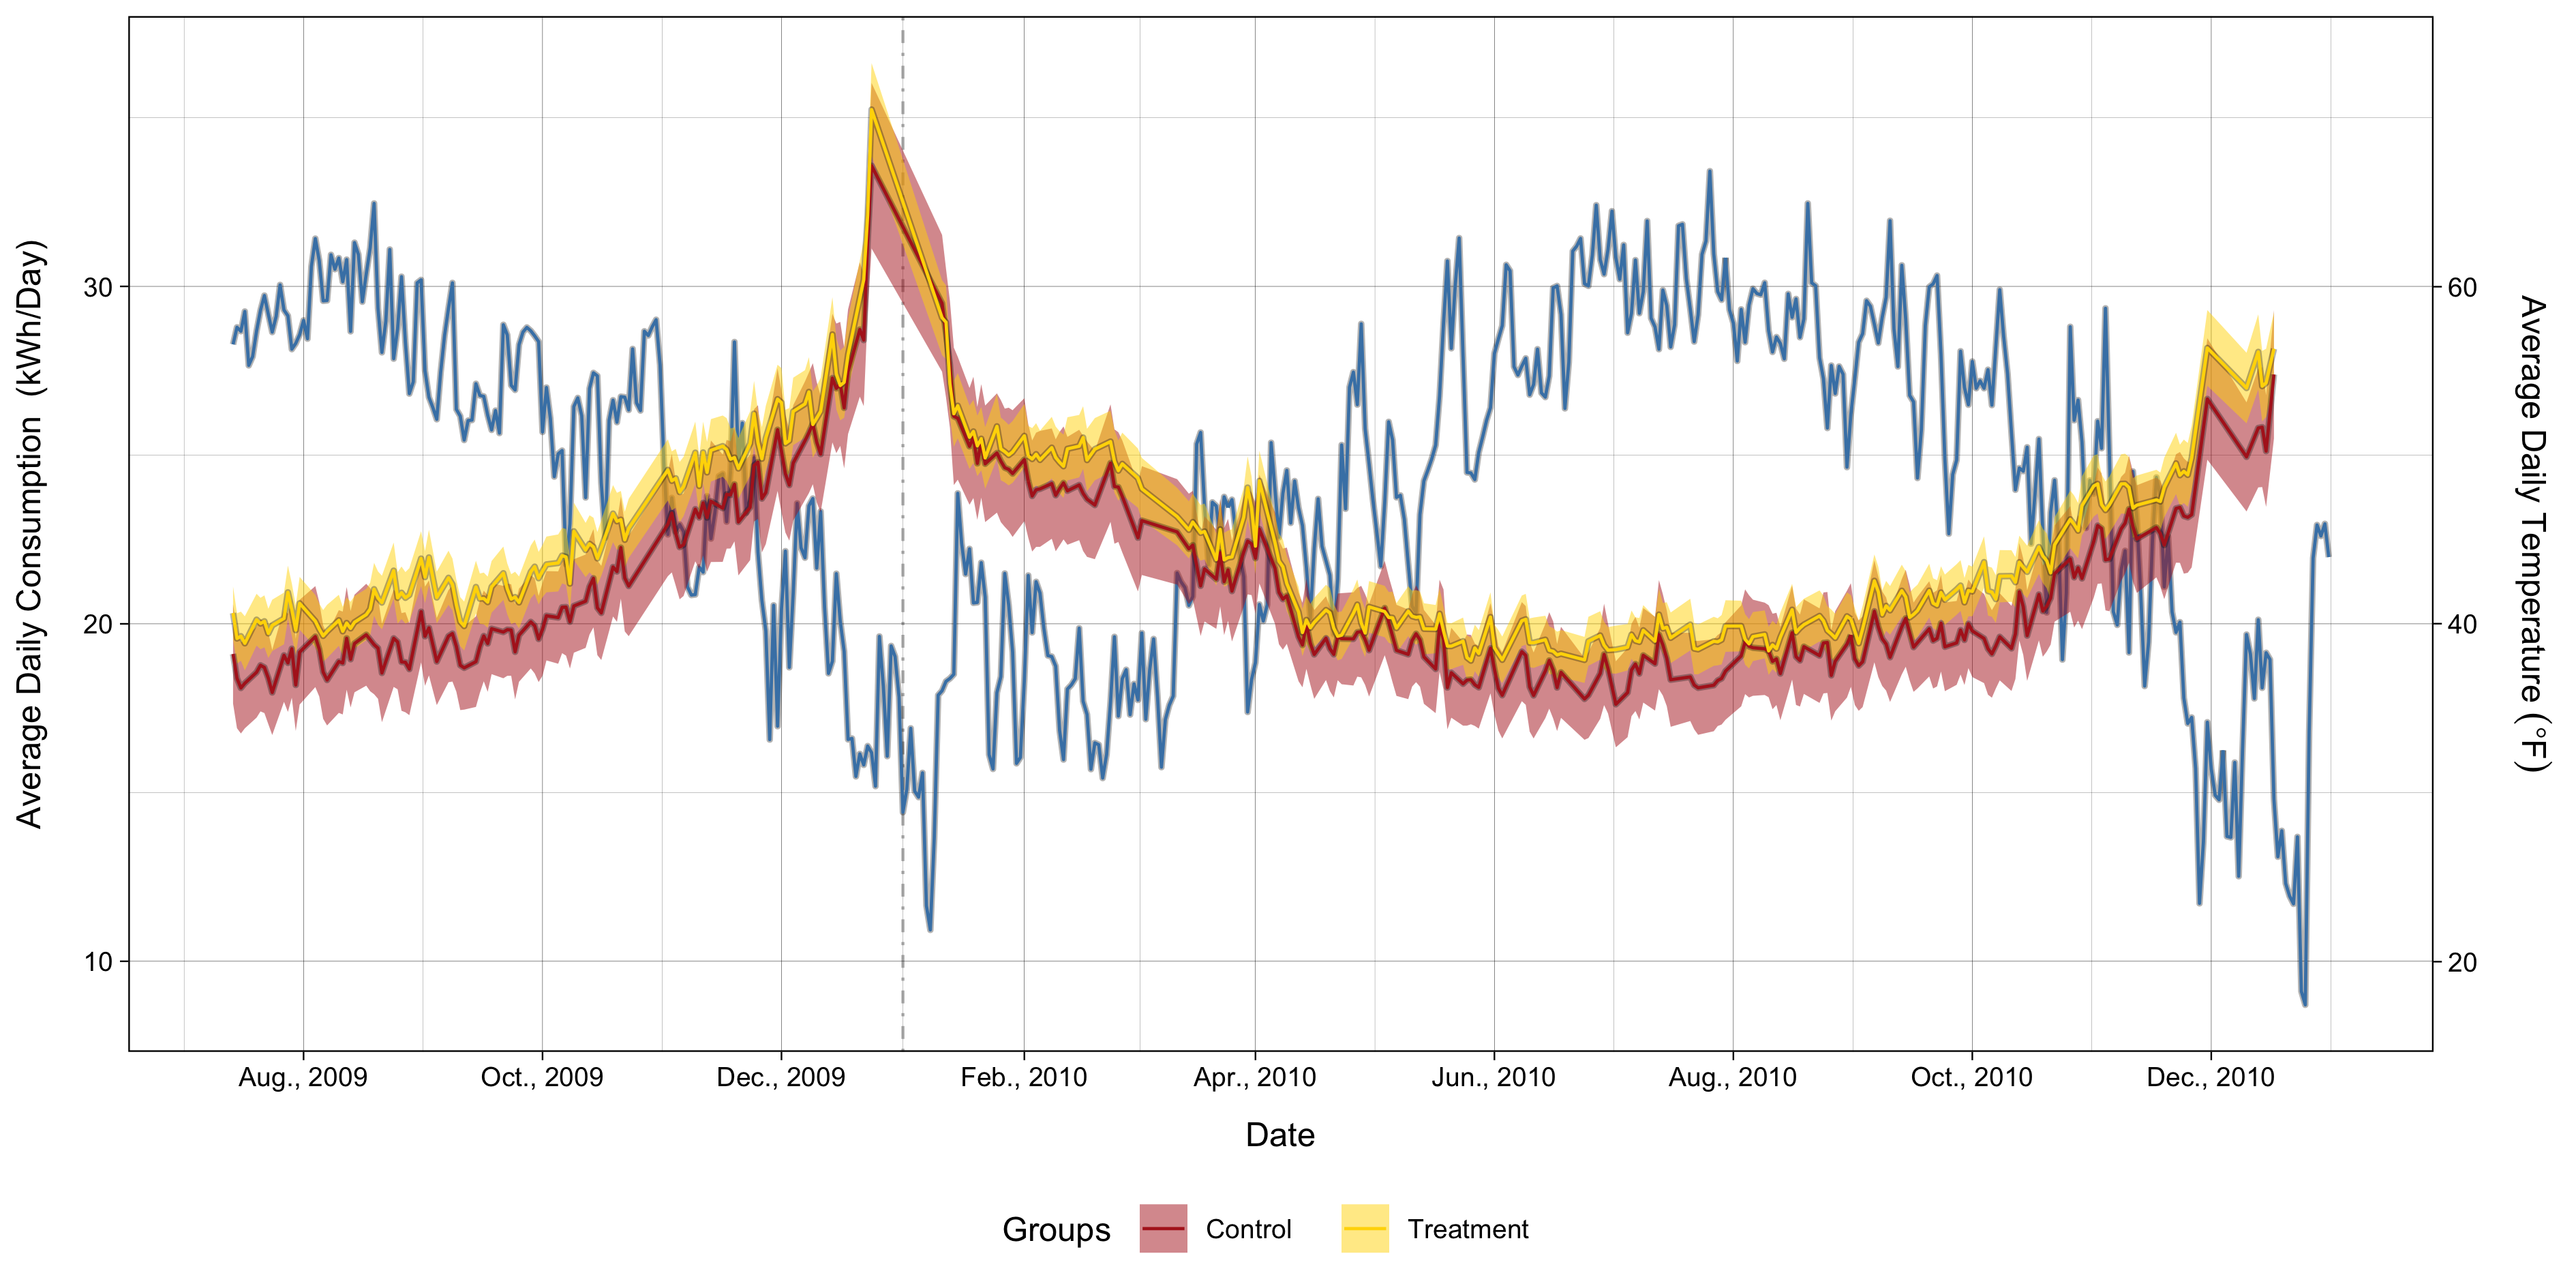
\includegraphics[scale = 0.11]{03_Chapter-2/00A_Figures/Figure_Average-Electricity-Consumption_Average-Daily-Consumption-by-Date.png}
%        \caption{Average Daily Electricity Consumption}
%        \subcaption*{\textit{Note}: The figure depicts not only the average daily electricity consumption of each group but also the average daily temperature. From this figure, it is explicit that household daily electricity consumption is negatively correlated with the average daily temperature.}
%        \label{Figure:Average-Daily-Electricity-Consumption}
%    \end{figure}
%%}
%\clearpage

%\afterpage{
    \begin{figure}[t!]
        \centering
        \includegraphics[scale = 0.032]{03_Chapter-2/00A_Figures/Figure_For-Motivation_Daily-Consumption-with-Percentage-Changes_Base-only-the-Second-Half_Step-Size-2.png}
        \caption{Pre- and Post-Treatment Household Average Daily Electricity Consumption}
%        \subcaption*{\textit{Note}: ...}
        \label{Figure:Pre-and-Post-Treatment-Household-Average-Daily-Electricity-Consumption}
    \end{figure}
%}
%\clearpage
\vspace{0.3cm}

%\afterpage{
    \begin{figure}
        \centering
        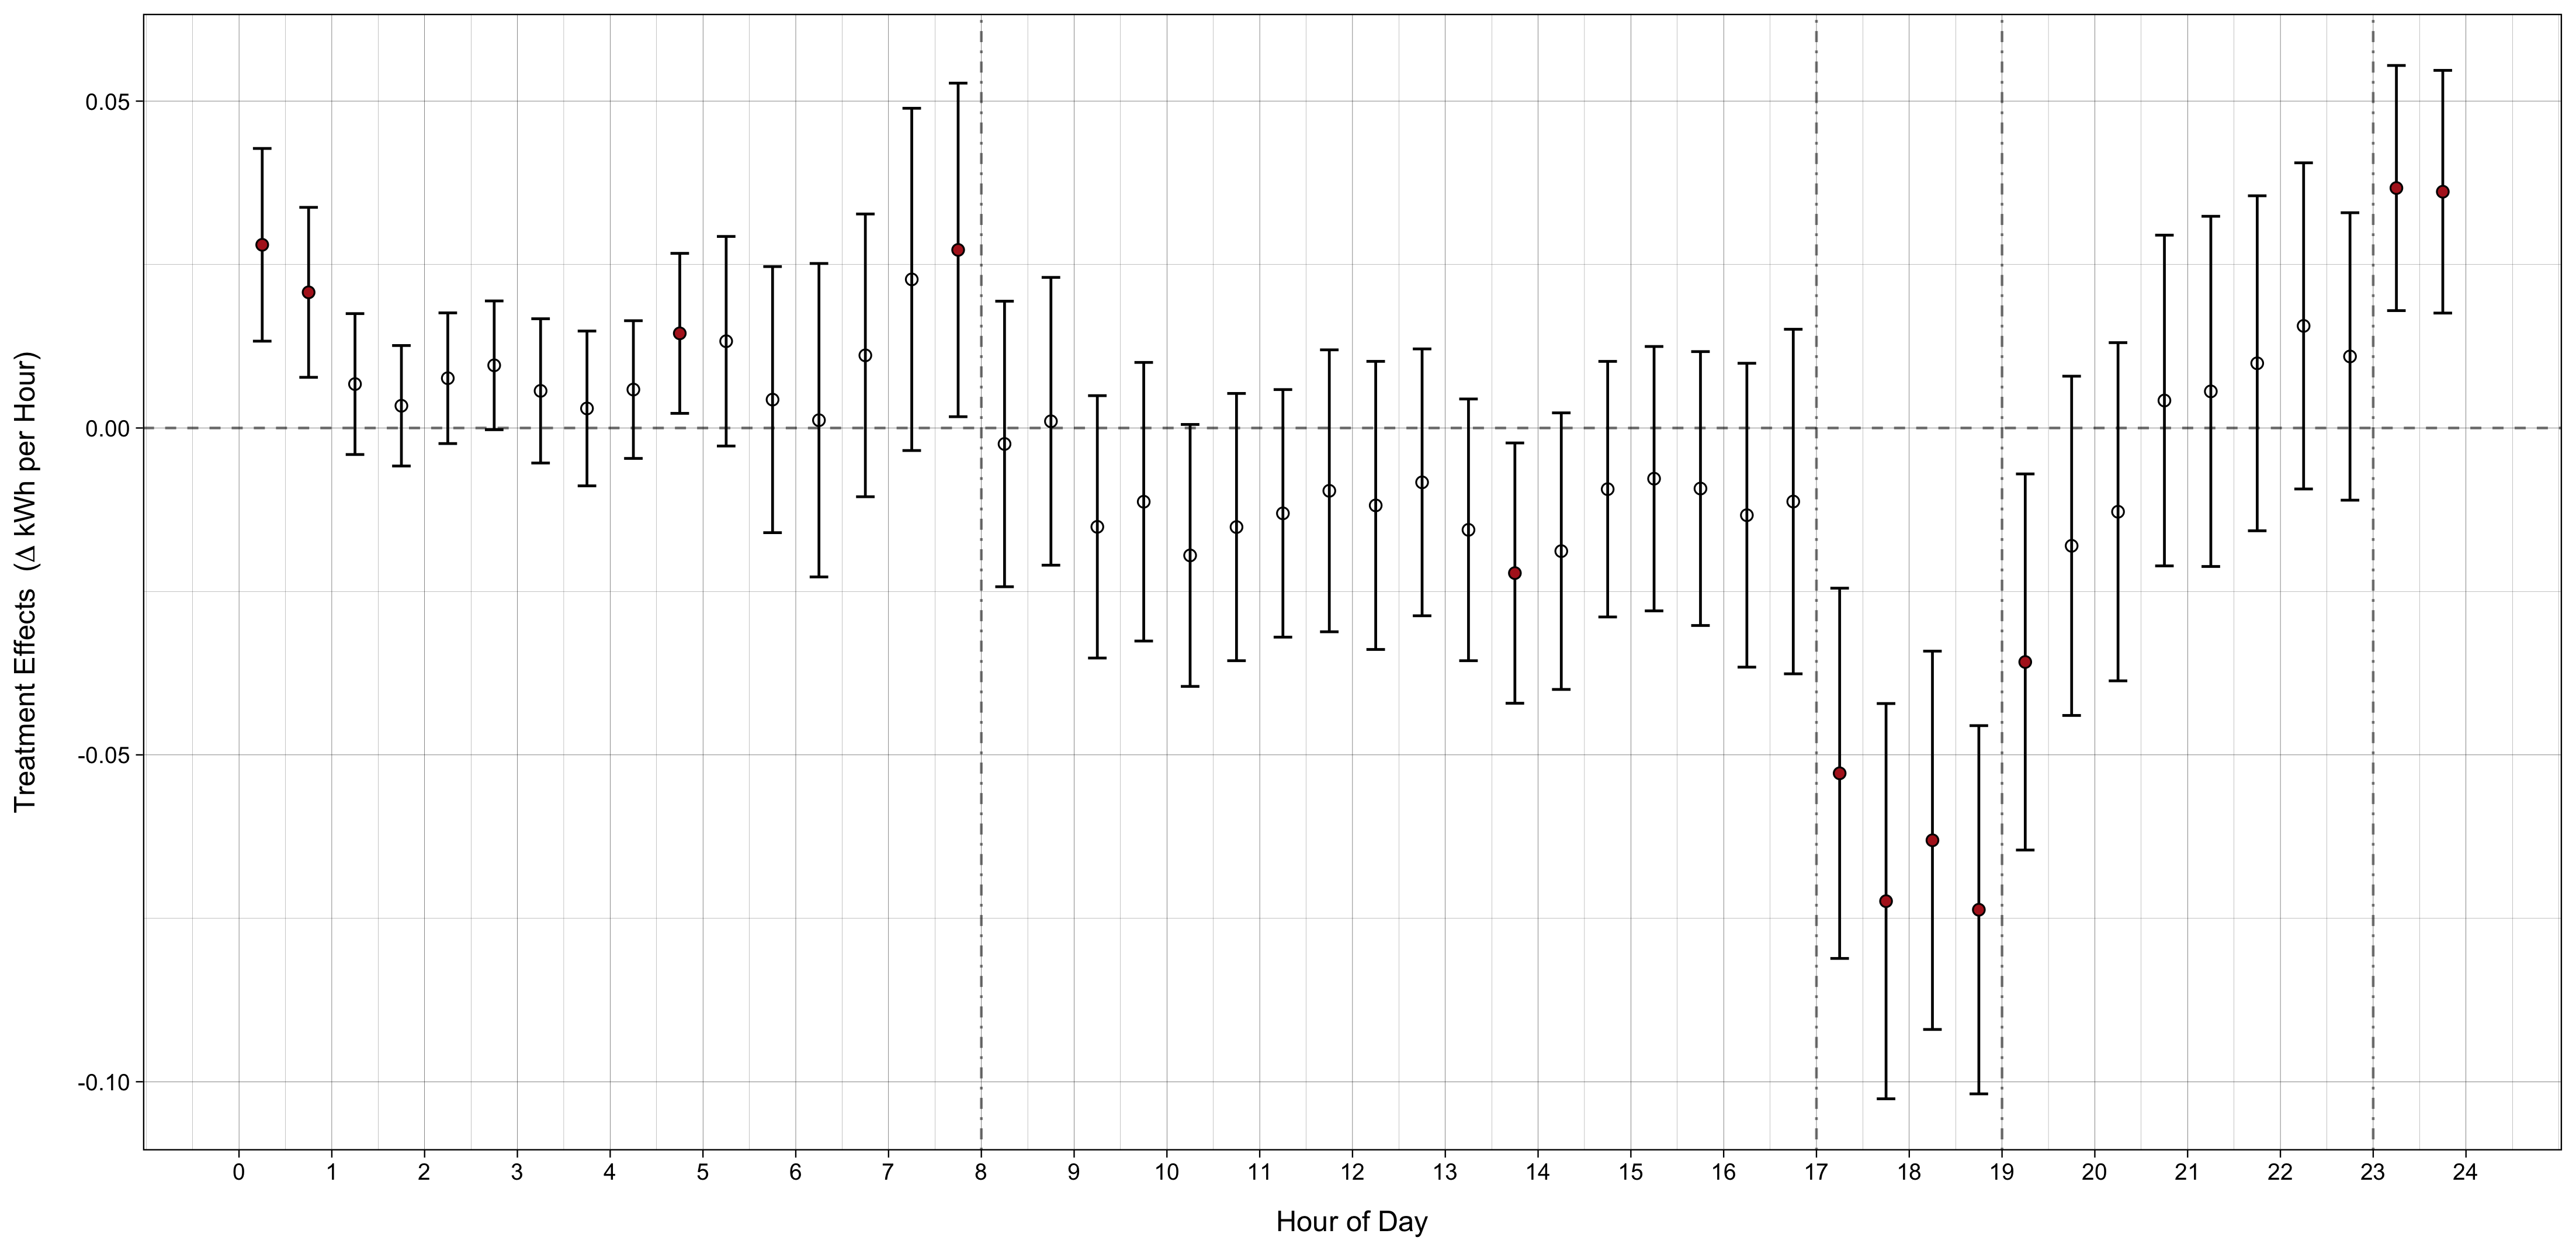
\includegraphics[scale = 0.10]{03_Chapter-2/00A_Figures/Figure_Time-Profile-of-Half-Hourly-ATEs.png}
        \caption{Half-Hourly Average Treatment Effects}
%        \subcaption*{\textit{Note}: ...}
        \label{Figure:Half-Hourly-Average-Treatment-Effects}
    \end{figure}
%}
%\clearpage
\hspace{0.3cm}

%\afterpage{
    \begin{figure}[t!]
        \centering
        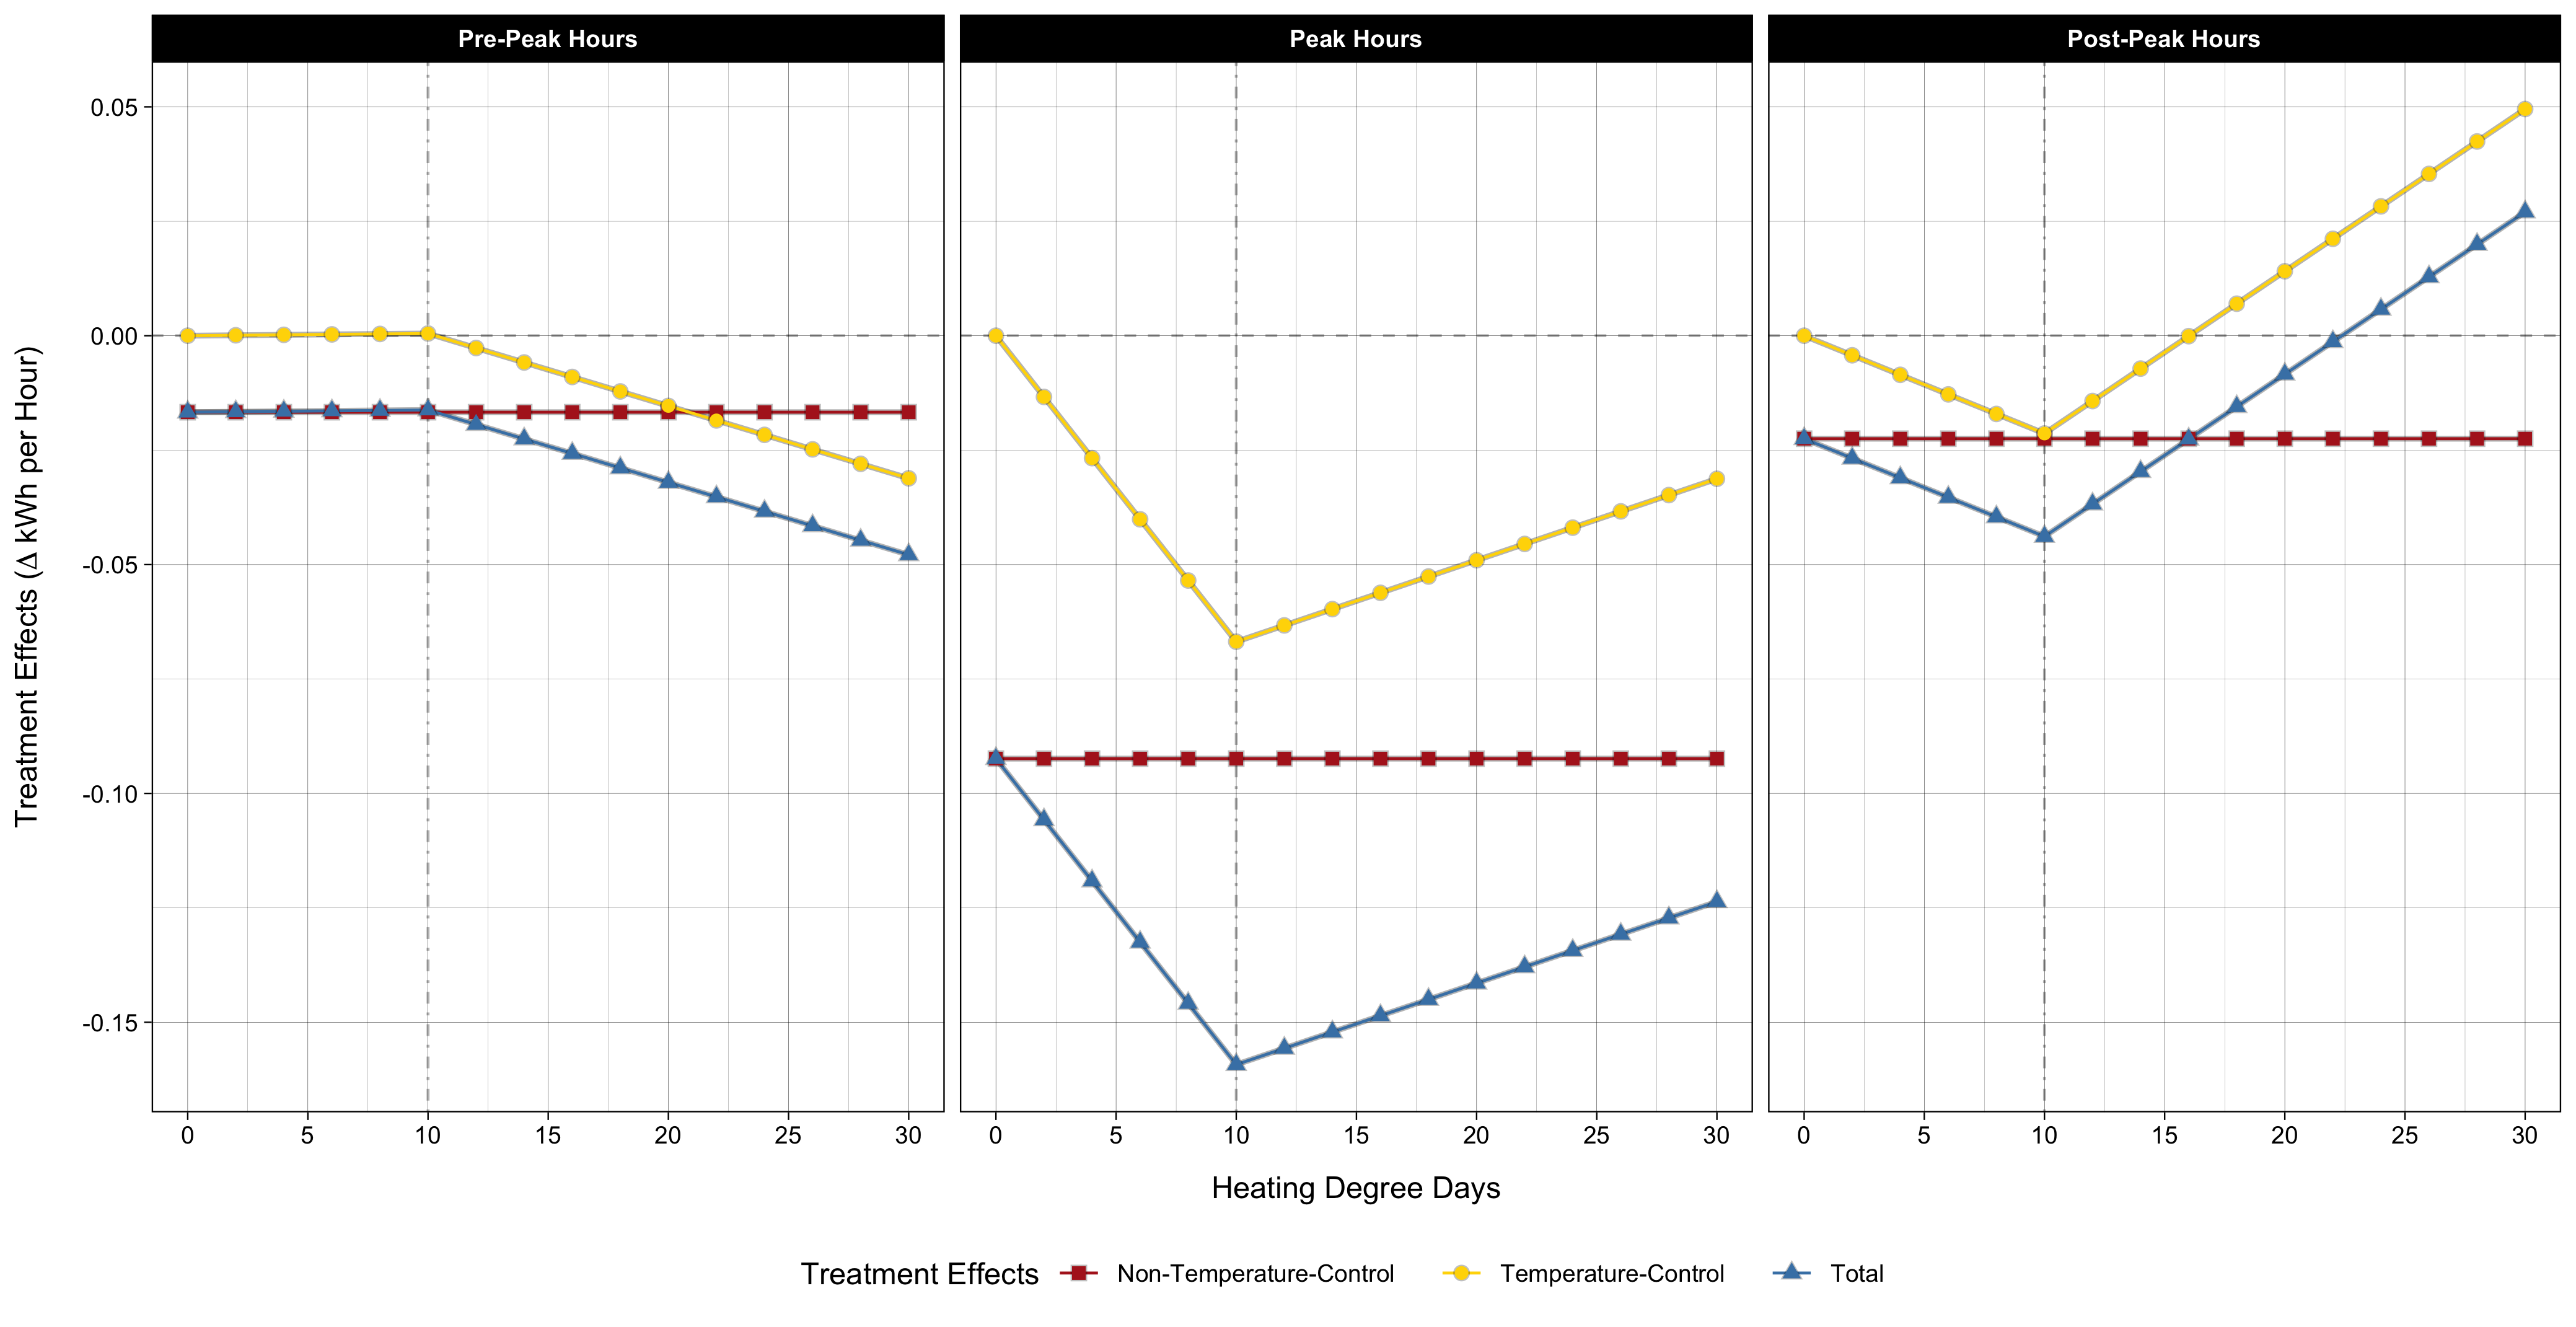
\includegraphics[scale = 0.1]{03_Chapter-2/00A_Figures/Figure_Breakdown-of-Hourly-ATEs_For-Different-Intervals_All_Knot-10.png}
        \caption{Breakdown of Hourly Average Treatment Effects}
%        \subcaption*{\textit{Note}: ...}
        \label{Figure:Breakdown-of-Hourly-ATEs-in-the-Peak-Rate-Period}
    \end{figure}
%}
%\clearpage
\vspace{0.3cm}

%\afterpage{
    \begin{figure}[t!]
        \centering
        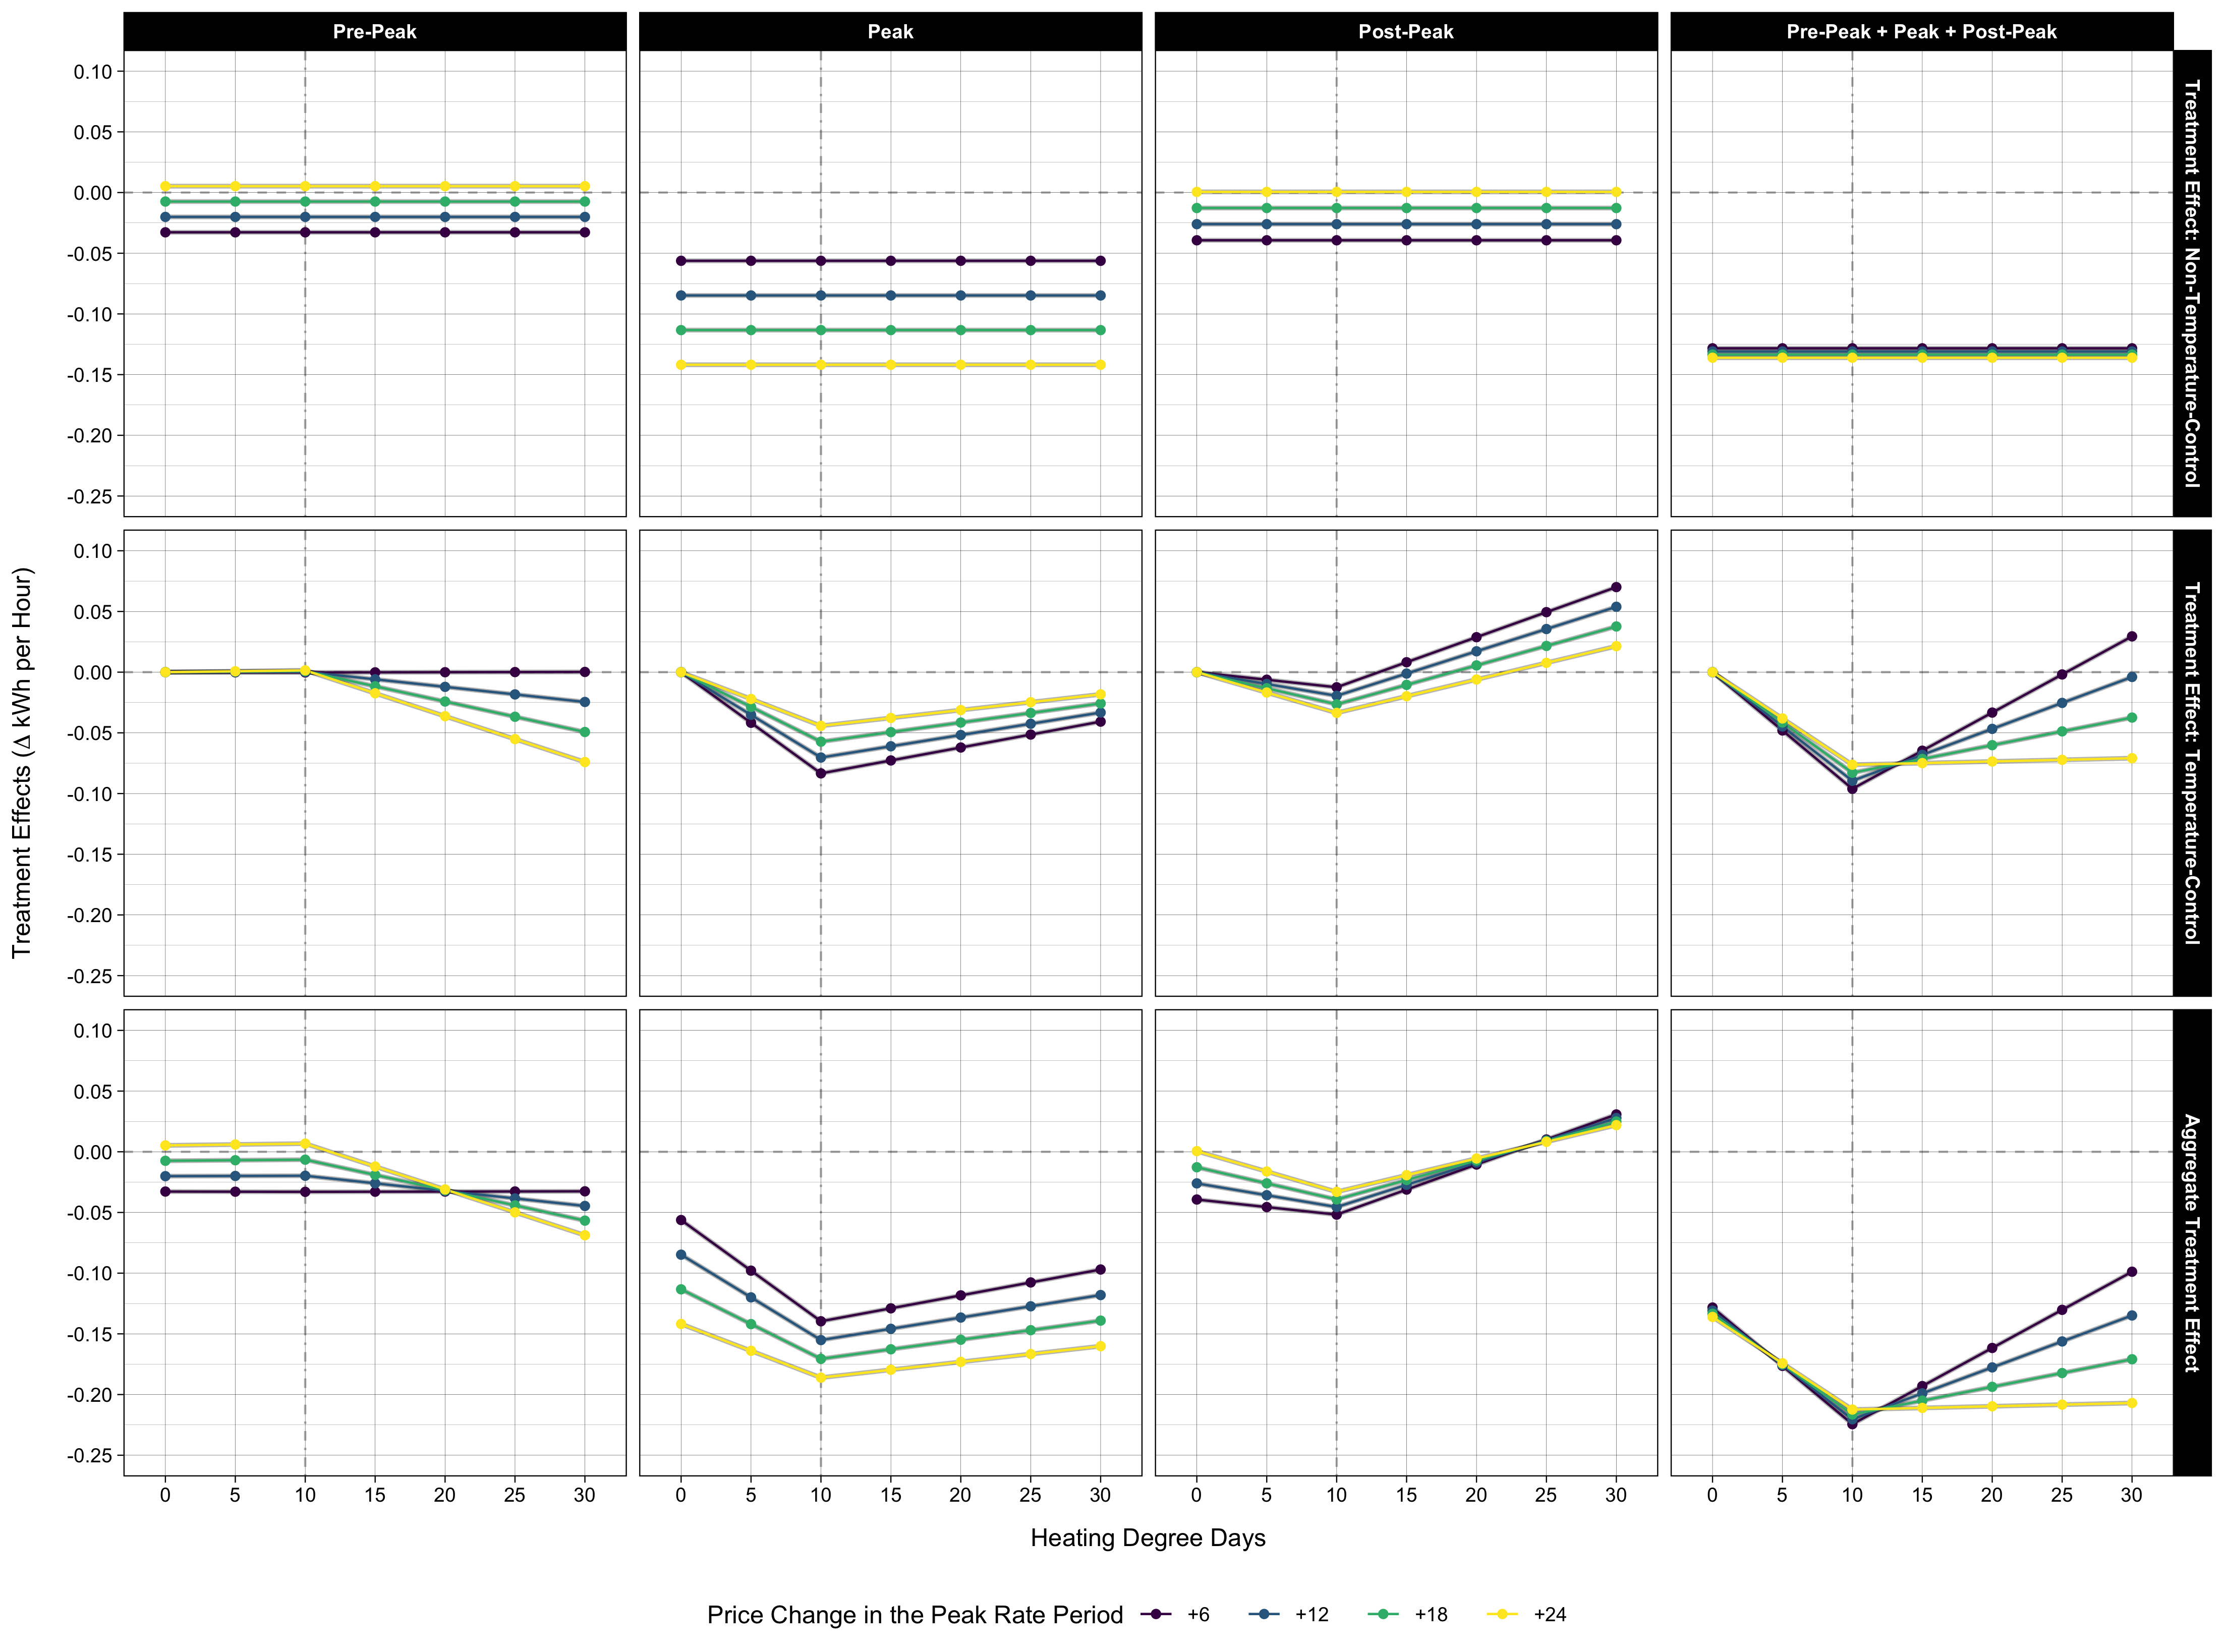
\includegraphics[scale = 0.09]{03_Chapter-2/00A_Figures/Figure_Predicted-Electricity-Savings_By-Intervals-and-HDDs_Spline_Knot-10.png}
        \caption{Treatment Effects as a Linear Function of Peak-hour Price Changes}
%        \subcaption*{\textit{Note}: ...}
        \label{Figure:Treatment-Effects-as-a-Linear-Function-of-Price-Changes-in-the-Peak-Rate-Period}
    \end{figure}
%}
%\clearpage
\hspace{0.3cm}

%\afterpage{
    \begin{figure}[t!]
        \centering
        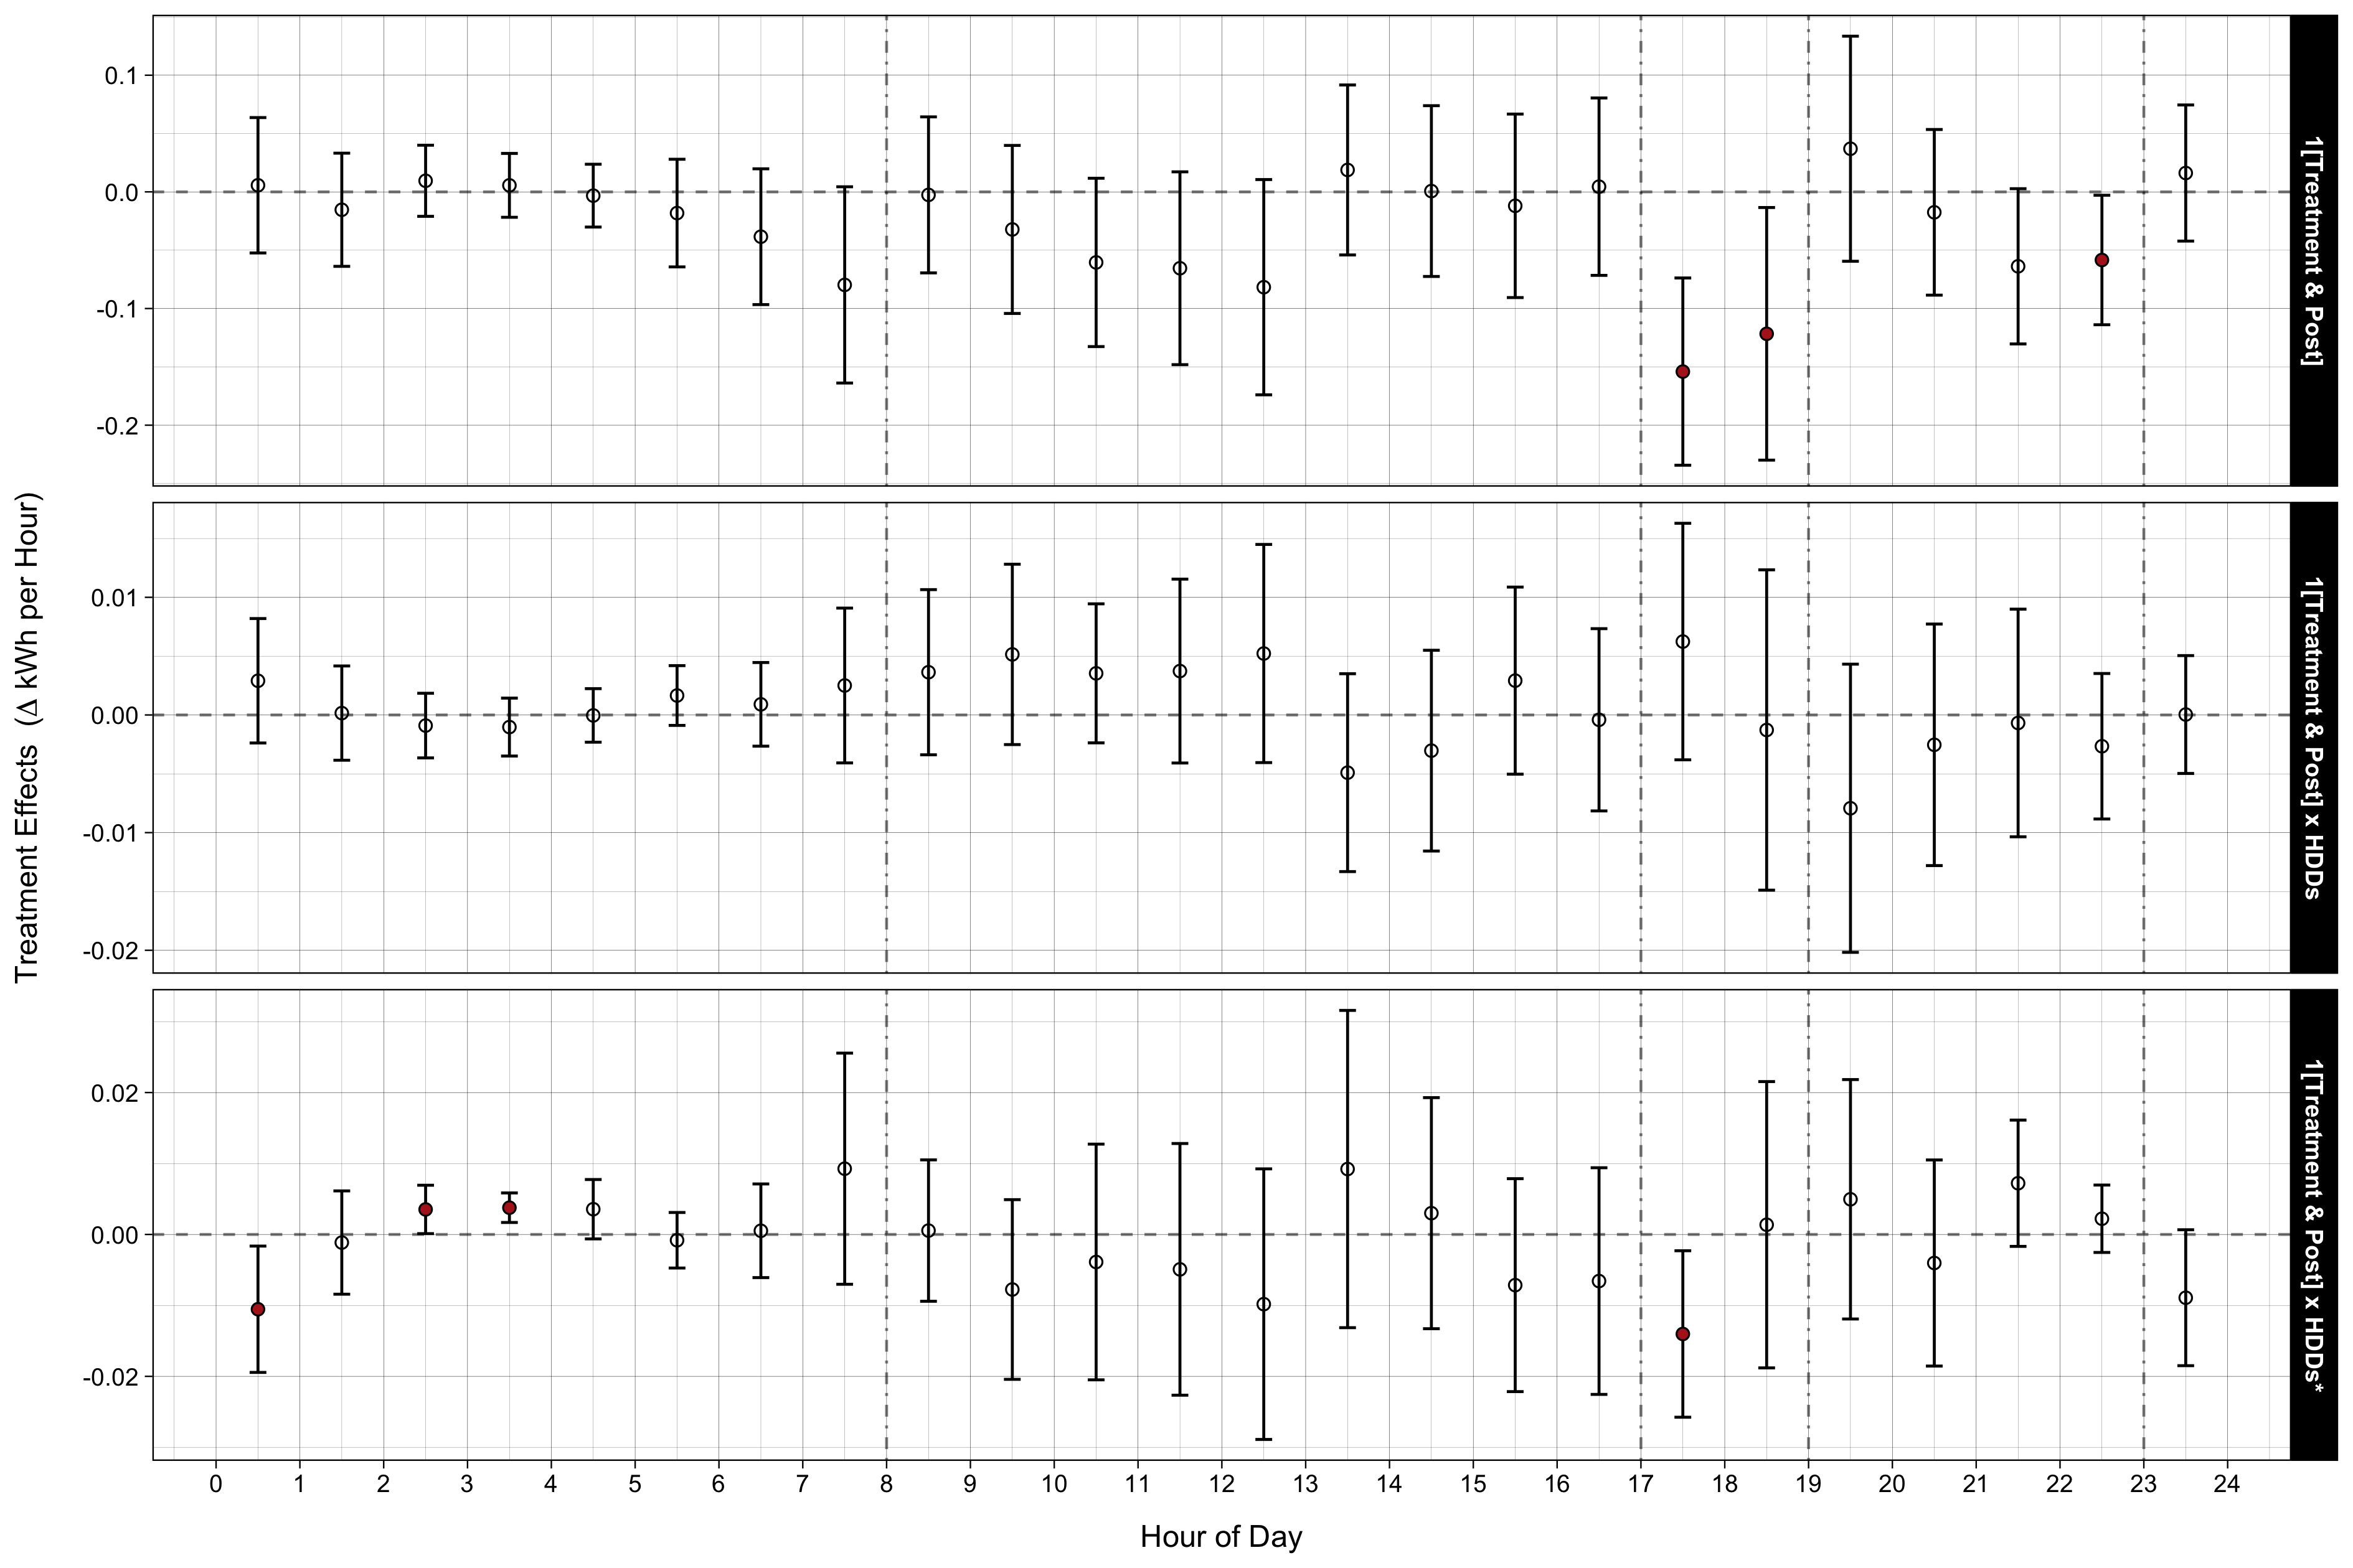
\includegraphics[scale = 0.1]{03_Chapter-2/00A_Figures/Figure_Time-Profile-of-ATEs_Using-Tariff-Groups-A-and-D_Knot-15.png}
        \caption{Relative Comparison of Tariff Group D to Tariff Group A}
%        \subcaption*{\textit{Note}: ...}
        \label{Figure:Relative-Comparison-of-Tariff-Group-D-to-Tariff-Group-A}
    \end{figure}
%}
%\clearpage
\hspace{0.3cm}

%\afterpage{
    \begin{figure}[t!]
        \centering
        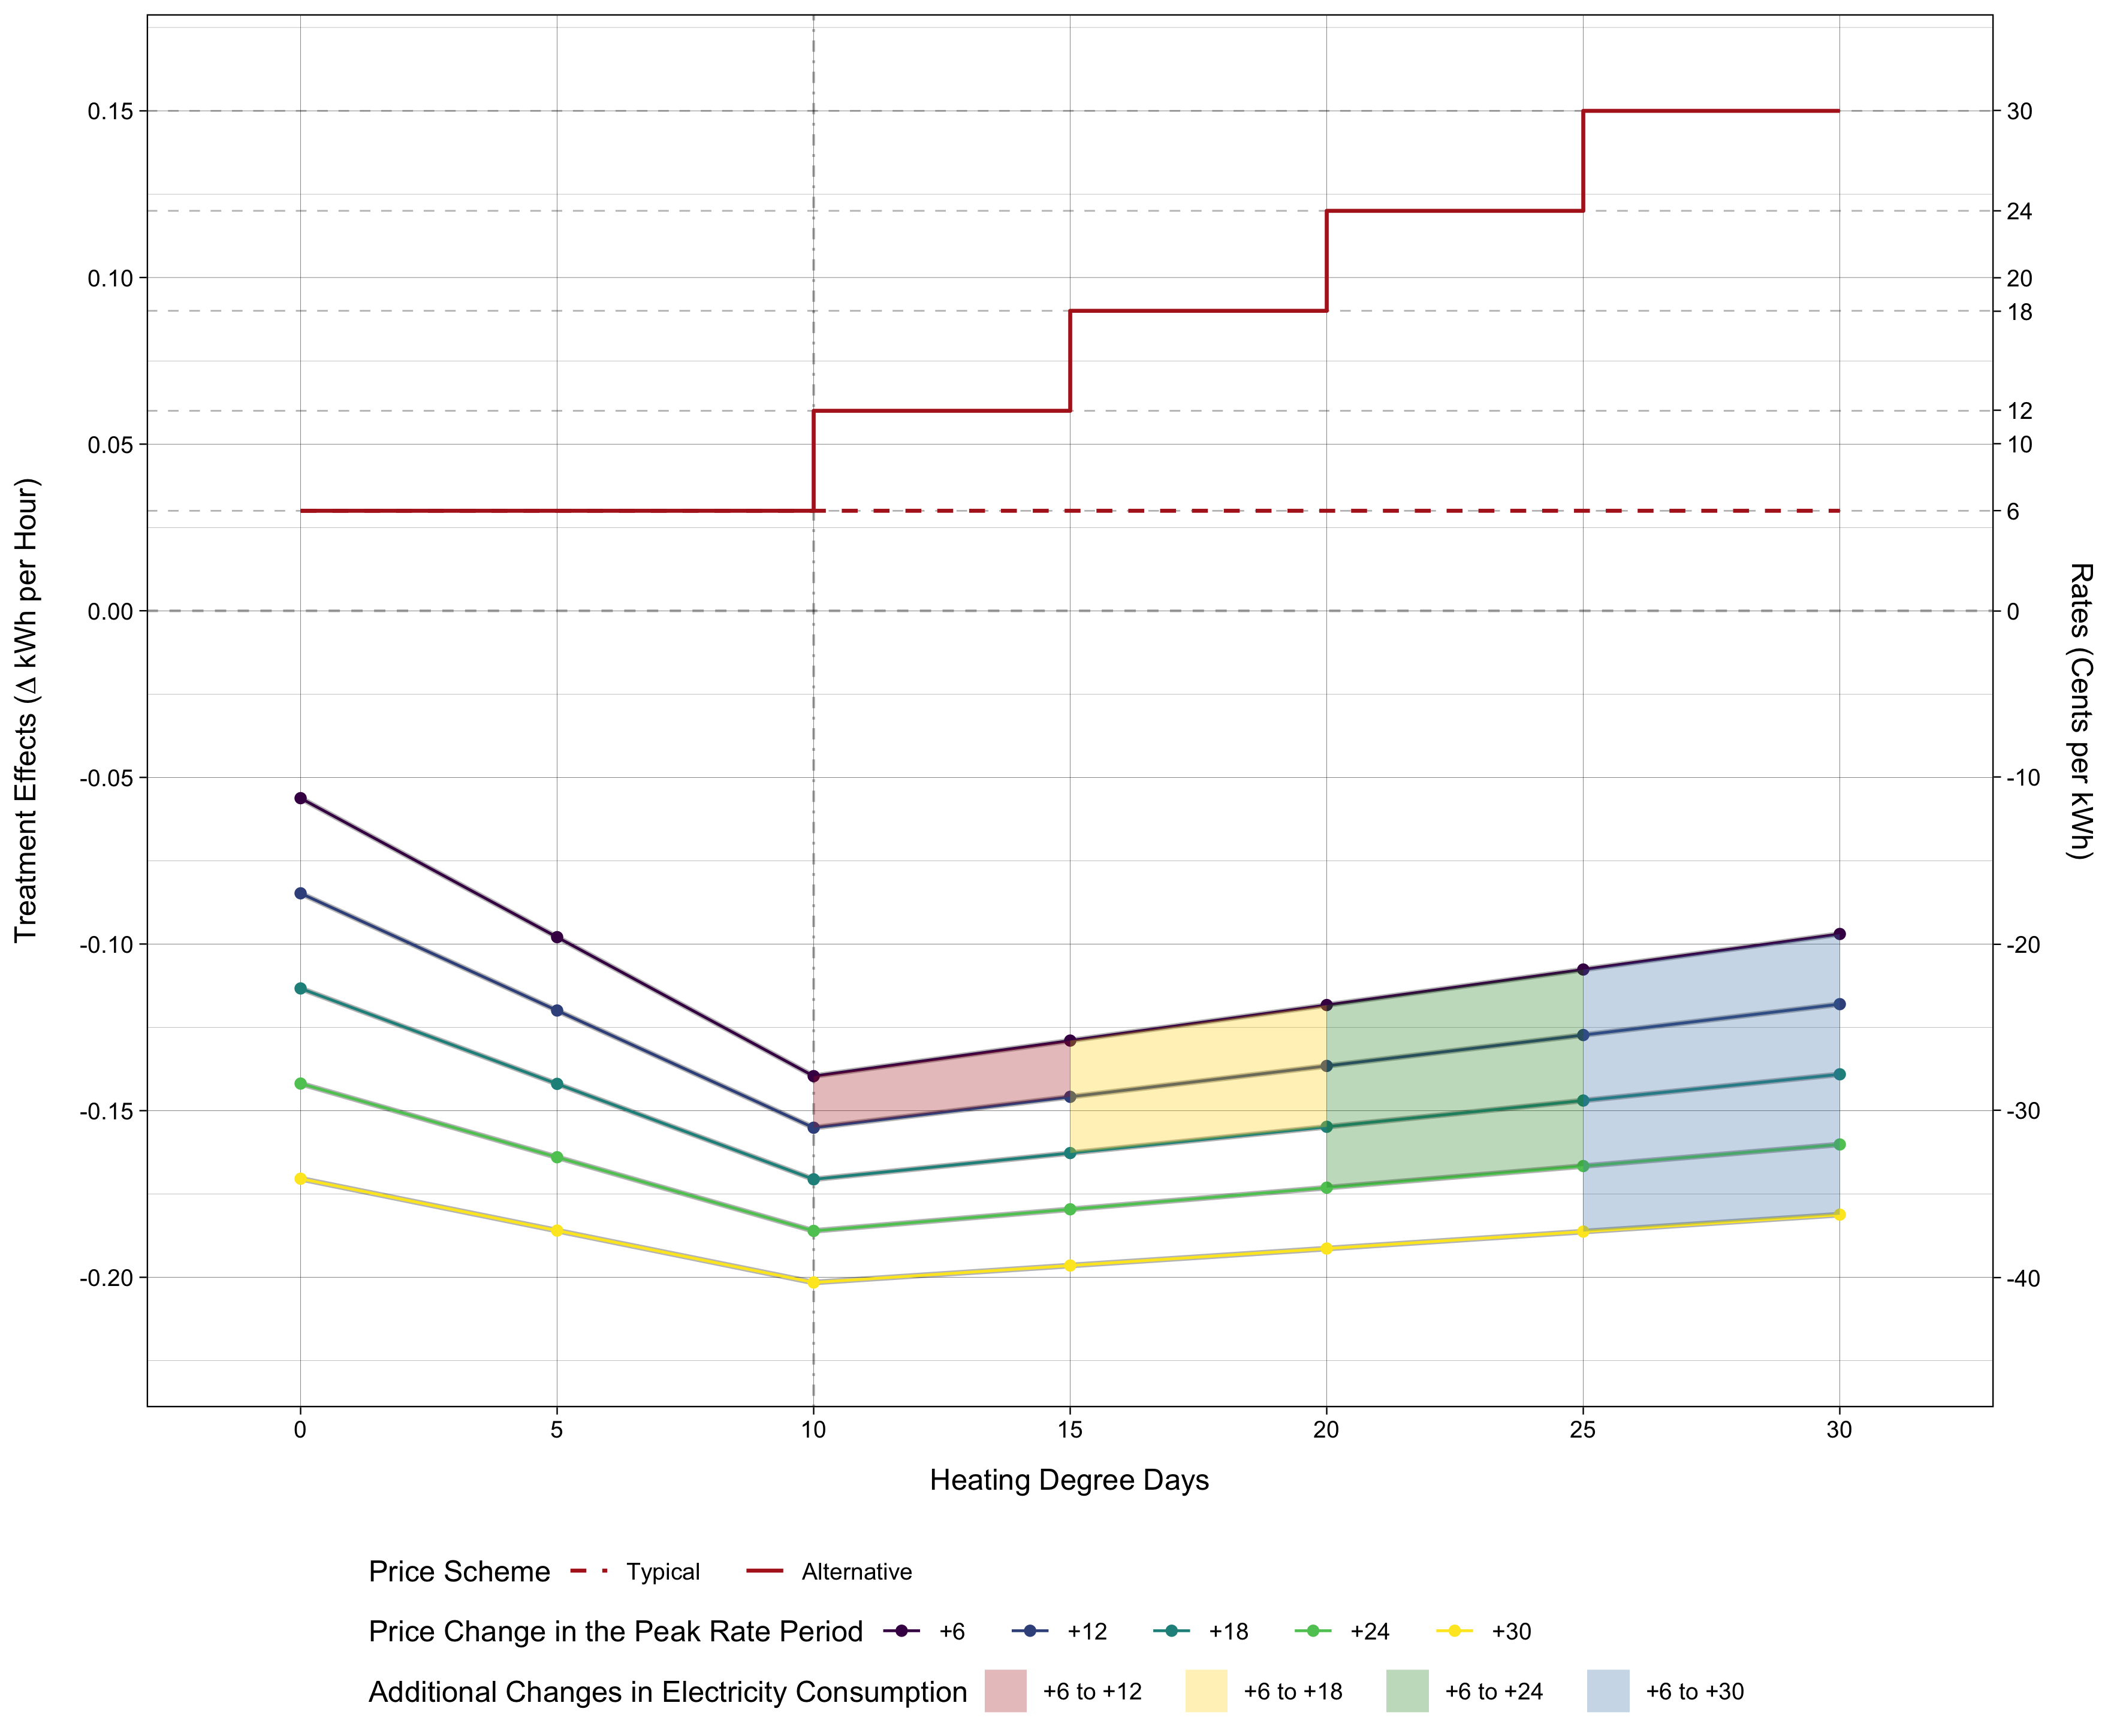
\includegraphics[scale = 0.075]{03_Chapter-2/00A_Figures/Figure_Additional-Electricity-Savings_Knot-10.png}
        \caption{Additional Gains from an Alternative Electricity Pricing Scheme}
%        \subcaption*{\textit{Note}: ...}
        \label{Figure:Additional-Savings-from-an-Alternative-Electricity-Pricing-Scheme}
    \end{figure}
%}
%\clearpage

% Tables
%\afterpage{
    \begin{table}
        \centering
        \caption{Summary Statistics and Differences in Means}
        \label{Table:Summary-Statistics-and-Differences-in-Means}
        \vspace{0.2cm}
        \begin{adjustbox}{scale = 0.9}
            \begin{tabular}{
                >{\raggedright}m{6.0cm}
                >{\raggedleft}m{1.25cm}
                >{\raggedleft}m{1.25cm}
                >{\raggedleft}m{0.1cm}
                >{\raggedleft}m{1.25cm}
                >{\raggedleft}m{1.25cm}
                >{\raggedleft}m{0.1cm}
                >{\raggedleft}m{1.25cm}
                >{\raggedleft}m{1.25cm}
                >{\raggedleft\arraybackslash}m{1.25cm}
            }
                \hline \hline
                \multicolumn{1}{c}{} & \multicolumn{2}{c}{Control} & \multicolumn{1}{c}{} & \multicolumn{2}{c}{Treatment} & \multicolumn{1}{c}{} & \multicolumn{3}{c}{Difference} \\
                \cline{2-3} \cline{5-6} \cline{8-10}
                \multicolumn{1}{c}{} & \multicolumn{1}{c}{Mean} & \multicolumn{1}{c}{(S.E.)} & \multicolumn{1}{c}{} & \multicolumn{1}{c}{Mean} & \multicolumn{1}{c}{(S.E.)} & \multicolumn{1}{c}{} & \multicolumn{1}{c}{Mean} & \multicolumn{1}{c}{(S.E.)} & \multicolumn{1}{c}{$p$-value} \\
                \hline
                \underline{Electricity Consumption during Baseline Period \ ($kWh$)} &  &  &  &  &  &  &  &  &  \\
                \hspace{0.2cm} Daily & 22.122 & (0.674) &  & 23.529 & (0.379) &  & 1.407 & (0.773) & 0.069 \\
                \hspace{0.2cm} Hourly & 0.939 & (0.028) &  & 0.996 & (0.016) &  & 0.057 & (0.032) & 0.074 \\
                \hspace{0.2cm} Hourly, Night Rate & 0.524 & (0.018) &  & 0.560 & (0.010) &  & 0.035 & (0.021) & 0.088 \\
                \hspace{0.2cm} Hourly, Day Rate & 1.128 & (0.034) &  & 1.193 & (0.019) &  & 0.065 & (0.039) & 0.095 \\
                \hspace{0.2cm} Hourly, Peak Rate & 1.537 & (0.053) &  & 1.642 & (0.029) &  & 0.105 & (0.060) & 0.080 \\
                \underline{Demographics} &  &  &  &  &  &  &  &  &  \\
                \hspace{0.2cm} Age Group: 65+? & 0.277 & (0.028) &  & 0.225 & (0.014) &  & -0.052 & (0.031) & 0.096 \\
                \hspace{0.2cm} Education: Third Level+? & 0.265 & (0.027) &  & 0.344 & (0.016) &  & 0.078 & (0.032) & 0.014 \\
                \hspace{0.2cm} Employed? & 0.488 & (0.031) &  & 0.596 & (0.016) &  & 0.108 & (0.035) & 0.002 \\
                \hspace{0.2cm} Number of People over 15 in Home & 2.488 & (0.061) &  & 2.506 & (0.032) &  & 0.019 & (0.077) & 0.808 \\
                \hspace{0.2cm} Number of People under 15 in Home & 1.754 & (0.060) &  & 1.964 & (0.035) &  & 0.210 & (0.138) & 0.132 \\
                \underline{Housing Characteristics} &  &  &  &  &  &  &  &  &  \\
                \hspace{0.2cm} Owned House? & 0.904 & (0.018) &  & 0.932 & (0.008) &  & 0.028 & (0.020) & 0.165 \\
                \hspace{0.2cm} Number of Bedrooms & 3.335 & (0.054) &  & 3.465 & (0.028) &  & 0.130 & (0.061) & 0.035 \\
                \hspace{0.2cm} Timer for Space Heating & 0.792 & (0.025) &  & 0.802 & (0.013) &  & 0.010 & (0.028) & 0.728 \\
                \hline \hline
            \end{tabular}
        \end{adjustbox}
        \begin{tablenotes}[flushleft]
            \small
            \textit{Note}: The variable descriptions with question mark suggest that these variables are binary.  
        \end{tablenotes}

    \end{table}
%}

\clearpage

%\afterpage{
    \begin{table}
        \centering
        \caption{Treatment and Control Group Assignments}
        \label{Table:Treatment-and-Control-Group-Assignments}
        \vspace{0.2cm}
        \begin{adjustbox}{scale = 1.0}
            \begin{tabular}{
                >{\raggedright}m{4.5cm} |
                >{\raggedleft}m{1.5cm} 
                >{\raggedleft}m{1.5cm} 
                >{\raggedleft}m{1.5cm} 
                >{\raggedleft}m{1.5cm} 
                >{\raggedleft}m{1.5cm} ||
                >{\raggedleft\arraybackslash}m{2.1cm}
            }
                \hline \hline
                \multicolumn{1}{c|}{Stimuli} & \multicolumn{5}{c||}{Tariffs} & \multicolumn{1}{c}{Total} \\
                \cline{2-6}
                \multicolumn{1}{c|}{}  & \multicolumn{1}{c}{Control} & \multicolumn{1}{c}{A} & \multicolumn{1}{c}{B} & \multicolumn{1}{c}{C} & \multicolumn{1}{c||}{D} & \multicolumn{1}{c}{} \\
                \hline
                Monthly Bill & 0 & 79 & 37 & 89 & 28 & 233 \\
                Bi-Monthly Bill & 0 & 81 & 34 & 76 & 34 & 225 \\
                Bi-Monthly Bill $+$ IHD & 0 & 79 & 22 & 86 & 30 & 217 \\
                Bi-Monthly Bill $+$ OLR & 0 & 90 & 27 & 84 & 34 & 235 \\
                Control & 260 & 0 & 0 & 0 & 0 & 260 \\
                \hline
                Total & 260 & 329 & 120 & 335 & 126 & 1,170 \\
                \hline \hline
            \end{tabular}
        \end{adjustbox}
%        \begin{tablenotes}[flushleft]
%            \small
%            \textit{Note}: (The purpose of this sentence is to determine the width of the table. Therefore, this note should be replaced or deleted after polishing the table size.)
%        \end{tablenotes}

    \end{table}
%}
\hspace{0.5cm}

%\afterpage{
    \begin{table}[ht!]
        \centering
        \caption{Breakdown of Hourly Average Treatment Effects}
        \label{Table:Breakdown-of-Hourly-ATEs_Coefficients-of-Interest-only}
        \vspace{0.3cm}
        \small
        \begin{adjustbox}{scale = 0.75}
            \begin{threeparttable}
                \begin{tabular}{@{\extracolsep{10pt}}lccccccc}
                    \\[-5.5ex]
                    \hline \hline
                    \\[-3.0ex]
%                    & \multicolumn{15}{c}{Dependent Variable} \\
%                    \\[-3.0ex]
%                    \cline{2-100}
%                    \\[-3.0ex]
                    & \multicolumn{7}{c}{Hourly Electricity Consumption  (kWh/Hour)} \\
                    \\[-3.0ex]
                    & (1) & (2) & (3) & (4) & (5) & (6) & (7) \\
                    \\[-3.0ex]
                    \hline
                    \\[-2.0ex]
                    $\mathbb{1}$[Treatment \& Post] & $-$0.018 & $-$0.096$^{***}$ & $-$0.030 & $-$0.056$^{**}$ & $-$0.128$^{***}$ & $-$0.086$^{***}$ & $-$0.194$^{***}$ \\
                    & (0.020) & (0.024) & (0.024) & (0.028) & (0.038) & (0.031) & (0.040) \\
                    & & & & & & & \\
                    $\mathbb{1}$[Treatment \& Post] $\times$ HDDs & 0.0002 & $-$0.005$^{**}$ & 0.0002 & $-$0.009$^{***}$ & $-$0.002 & $-$0.002 & $-$0.007 \\
                    & (0.002) & (0.002) & (0.002) & (0.003) & (0.003) & (0.003) & (0.005) \\
                    & & & & & & & \\
                    $\mathbb{1}$[Treatment \& Post] $\times$ HDDs$^{*}$ & $-$0.003 & 0.010$^{***}$ & 0.003$^{*}$ & 0.019$^{***}$ & 0.003 & 0.003 & 0.013$^{**}$ \\
                    & (0.004) & (0.002) & (0.002) & (0.003) & (0.004) & (0.002) & (0.005) \\
                    & & & & & & & \\
                    \hline
                    \\[-2.0ex]
                    Tariff Group & All & All & All & A & B & C & D \\
                    Description of Interval & Pre-Peak & Peak & Post-Peak & Peak & Peak & Peak & Peak \\
                    Interval of Hours & 15 to 16 & 17 to 18 & 19 to 20 & 17 to 18 & 17 to 18 & 17 to 18 & 17 to 18 \\
                    Knot & 15 & 15 & 15 & 15 & 15 & 15 & 15 \\
                    FEs: Day of Week by Half-Hourly Time Window & Yes & Yes & Yes & Yes & Yes & Yes & Yes \\
                    Observations & 1,006,200 & 1,006,200 & 1,006,200 & 506,540 & 326,800 & 511,700 & 331,960 \\
                    Adjusted R$^{2}$ & 0.024 & 0.047 & 0.040 & 0.046 & 0.045 & 0.044 & 0.045 \\
                    \\[-2.0ex]
                    \hline \hline
                    \\[-4.5ex]
                \end{tabular}
                \begin{tablenotes}[flushleft]
                    \footnotesize
                    \item \textit{Note}: * $p < 0.1$, ** $p < 0.05$, and *** $p < 0.01$.
                \end{tablenotes}
            \end{threeparttable}
        \end{adjustbox}
    \end{table}
%}

\clearpage

\afterpage{
    \begin{sidewaystable}[t!]
        \centering
        \caption{Hourly Average Treatment Effects in and near the Peak Rate Period}
        \label{Table:Hourly-Average-Treatment-Effects-in-and-near-the-Peak-Rate-Period}
        \small
        \begin{adjustbox}{scale = 0.65}
            \begin{threeparttable}
                \begin{tabular}{@{\extracolsep{1pt}}lccccccccccccccc}
                    \\[-5.5ex]
                    \hline \hline
                    \\[-3.0ex]
%                    & \multicolumn{15}{c}{Dependent Variable} \\
%                    \\[-3.0ex]
%                    \cline{2-16}
%                    \\[-3.0ex]
                    & \multicolumn{15}{c}{Hourly Electricity Consumption  (kWh/Hour)} \\
                    \\[-3.0ex]
                    & (1) & (2) & (3) & (4) & (5) & (6) & (7) & (8) & (9) & (10) & (11) & (12) & (13) & (14) & (15)\\
                    \\[-3.0ex]
                    \hline
                    \\[-2.0ex]
                    $\mathbb{1}$[Treatment \& Post] & $-$0.048$^{***}$ & $-$0.053$^{*}$ & $-$0.002 & $-$0.049 & $-$0.032$^{***}$ & $-$0.125$^{***}$ & $-$0.161$^{***}$ & $-$0.119$^{***}$ & $-$0.249$^{***}$ & $-$0.143$^{***}$ & $-$0.082$^{***}$ & $-$0.055$^{*}$ & $-$0.015 & $-$0.113$^{**}$ & $-$0.058$^{***}$ \\
                    & (0.016) & (0.027) & (0.017) & (0.031) & (0.011) & (0.020) & (0.036) & (0.022) & (0.044) & (0.015) & (0.020) & (0.030) & (0.021) & (0.048) & (0.015) \\
                    & & & & & & & & & & & & & & & \\
                    \hline
                    \\[-2.0ex]
                    Description of Interval & Pre-Peak & Pre-Peak & Pre-Peak & Pre-Peak & Pre-Peak & Peak & Peak & Peak & Peak & Peak & Post-Peak & Post-Peak & Post-Peak & Post-Peak & Post-Peak \\
                    Interval of Hours & 15 to 16 & 15 to 16 & 15 to 16 & 15 to 16 & 15 to 16 & 17 to 18 & 17 to 18 & 17 to 18 & 17 to 18 & 17 to 18 & 19 to 20 & 19 to 20 & 19 to 20 & 19 to 20 & 19 to 20 \\
                    Tariff Group & A & B & C & D & All & A & B & C & D & All & A & B & C & D & All \\
                    FEs: Household by Half-Hourly Time Window & Yes & Yes & Yes & Yes & Yes & Yes & Yes & Yes & Yes & Yes & Yes & Yes & Yes & Yes & Yes \\
                    FEs: Day of Week by Half-Hourly Time Window & Yes & Yes & Yes & Yes & Yes & Yes & Yes & Yes & Yes & Yes & Yes & Yes & Yes & Yes & Yes \\
                    FEs: Month of Year & Yes & Yes & Yes & Yes & Yes & Yes & Yes & Yes & Yes & Yes & Yes & Yes & Yes & Yes & Yes \\
                    Observations & 506,540 & 326,800 & 511,700 & 331,960 & 1,006,200 & 506,540 & 326,800 & 511,700 & 331,960 & 1,006,200 & 506,540 & 326,800 & 511,700 & 331,960 & 1,006,200 \\
                    Adjusted R$^{2}$ & 0.312 & 0.330 & 0.320 & 0.327 & 0.308 & 0.384 & 0.397 & 0.383 & 0.367 & 0.379 & 0.371 & 0.389 & 0.376 & 0.361 & 0.372 \\
                    \\[-2.0ex]
                    \hline \hline
                    \\[-4.5ex]
                \end{tabular}
                \begin{tablenotes}[flushleft]
                    \footnotesize
                    \item \textit{Note}: * $p < 0.1$, ** $p < 0.05$, and *** $p < 0.01$.
                \end{tablenotes}
            \end{threeparttable}
        \end{adjustbox}
    \end{sidewaystable}
}
    
\clearpage

%%\afterpage{
    \begin{table}[t!]
        \centering
        \caption{Correlations in Average Daily Temperatures between Weather Stations}
        \label{Table:Correlations-in-Average-Daily-Temperatures-among-Weather-Stations}
        \vspace{0.2cm}
        \begin{adjustbox}{scale = 0.75}
            \begin{tabular}{
                >{\raggedright}m{4.8cm} |
                >{\centering}m{5.5cm} 
                >{\centering\arraybackslash}m{5.5cm}
            }
                \hline \hline
                \multicolumn{1}{c|}{Stations} & \multicolumn{2}{c}{Correlation Coefficients} \\
                \cline{2-3}
                \multicolumn{1}{c|}{}  & \multicolumn{1}{c}{For Sample Period} & \multicolumn{1}{c}{For Experiment Period} \\
                \hline
                Ballyhaise & 0.98291 & 0.98244 \\
                Belmullet & 0.96089 & 0.96361 \\
                Cork Airport & 0.97121 & 0.97130 \\
                Gurteen & 0.98389 & 0.98307 \\
                Johnstown & 0.98189 & 0.97958 \\
                Mace & 0.95870 & 0.95921 \\
                Malin & 0.95632 & 0.95705 \\
                Markree Castle & 0.97194 & 0.97179 \\
                Moore Park & 0.98057 & 0.97798 \\
                Mount Dillon & 0.97945 & 0.97782 \\
                Mullingar & 0.98876 & 0.98654 \\
                Newport Furnace & 0.97015 & 0.97211 \\
                Oak Park & 0.99074 & 0.98925 \\
                Shannon Airport & 0.97696 & 0.97582 \\
                Sherkin Island & 0.95342 & 0.95411 \\
                \hline \hline
            \end{tabular}
        \end{adjustbox}
%        \begin{tablenotes}[flushleft]
%            \small
%            \item \textit{Note}: For each weather station, historical weather data from the weather station at Dublin airport is utilized to compute the two correlation coefficients. I do not provide the $p$-value of each correlation coefficient because it is arbitrarly small in magnitude. And the experiment period is the period between July 2009 to December 2010, while the sample period is the second half of 2009 and 2010. 
%        \end{tablenotes}
    \end{table}
%}

%\hspace{0.5cm}


\afterpage{
    \begin{table}[t!]
        \centering
        \caption{Hourly Treatment Effects as a Linear Function of Peak-Rate-Period Price Changes}
        \label{Table:Hourly-ATEs-as-a-Linear-Function-of-Peak-Rate-Period-Price-Changes_Coefficients-of-Interest-only}
        \vspace{0.3cm}
        \small
        \begin{adjustbox}{scale = 1.0}
            \begin{threeparttable}
                \begin{tabular}{@{\extracolsep{40pt}}lccc}
                    \\[-5.5ex]
                    \hline \hline
                    \\[-3.0ex]
%                    & \multicolumn{15}{c}{Dependent Variable} \\
%                    \\[-3.0ex]
%                    \cline{2-100}
%                    \\[-3.0ex]
                    & \multicolumn{3}{c}{Hourly Electricity Consumption  (kWh/Hour)} \\
                    \\[-3.0ex]
                    & (1) & (2) & (3) \\
                    \\[-3.0ex]
                    \hline
                    \\[-2.0ex]
                    $\mathbb{1}$[Treatment \& Post] & $-$0.045 & $-$0.028 & $-$0.053 \\
                    & (0.029) & (0.035) & (0.035) \\
                    & & & \\
                    $\mathbb{1}$[Treatment \& Post] $\times$ $\Delta$PC & 0.002 & $-$0.005$^{**}$ & 0.002 \\
                    & (0.002) & (0.002) & (0.002) \\
                    & & & \\
                    $\mathbb{1}$[Treatment \& Post] $\times$ HDDs & $-$0.0001 & $-$0.010$^{**}$ & $-$0.001 \\
                    & (0.004) & (0.004) & (0.004) \\
                    & & & \\
                    $\mathbb{1}$[Treatment \& Post] $\times$ HDDs$^{*}$ & 0.001 & 0.012$^{**}$ & 0.005 \\
                    & (0.005) & (0.006) & (0.005) \\
                    & & & \\
                    $\mathbb{1}$[Treatment \& Post] $\times$ HDDs $\times$ $\Delta$PC & 0.00001 & 0.0002 & $-$0.0001 \\
                    & (0.0002) & (0.0002) & (0.0003) \\
                    & & & \\
                    $\mathbb{1}$[Treatment \& Post] $\times$ HDDs$^{*}$ $\times$ $\Delta$PC & $-$0.0002 & $-$0.0003 & 0.00004 \\
                    & (0.0003) & (0.0003) & (0.0003) \\
                    & & & \\
                    \hline
                    \\[-2.0ex]
                    Description of Period & Pre-Peak & Peak & Post-Peak \\
                    Period of Hours & 15 to 16 & 17 to 18 & 19 to 20 \\
                    Knot & 10 & 10 & 10 \\
                    FEs: Day of Week by Half-Hourly Time Window & Yes & Yes & Yes \\
                    Observations & 1,006,200 & 1,006,200 & 1,006,200 \\
                    Adjusted R$^{2}$ & 0.024 & 0.047 & 0.040 \\
                    \\[-2.0ex]
                    \hline \hline
                    \\[-4.5ex]
                \end{tabular}
                \begin{tablenotes}[flushleft]
                    \footnotesize
                    \item \textit{Note}: * $p < 0.1$, ** $p < 0.05$, and *** $p < 0.01$.
                \end{tablenotes}
            \end{threeparttable}
        \end{adjustbox}
    \end{table}
}

